\documentclass[a4paper,11pt,twocolumn]{article}
\usepackage{tikz}

\title{
  Panzergruppe Guderian: \\
  THE BATTLE OF SMOLENSK, JULY 1941
}

\author{This document created by: Daniel Berger - \today}

\date{}

\setlength{\columnsep}{2em}
\setcounter{tocdepth}{2}

\begin{document}
  \maketitle
  \tableofcontents
  \section{INTRODUCTION}

\textbf{Panzergruppe Guderian} is a regimental/divisional level simulation of the German drive to cross the Dnepr River in the summer of 1941 and seize the valuable communications junctions at Smolensk in preparation for the final push towards Moscow. Each turn is equivalent to two days of real time and each hex equals 10.5 kilometers.

Section 2.0 of the rules gives the Players a general course of play; it takes the reader through a narrative description of the rules, giving a general outline of how the game works and how it progresses. Experienced Players will find they can usually proceed to play right from this section, using the specific rules as references. The new gamer will find this section useful in initiating him to the flow of play.
  \begin{flushleft}
  \section{HOW TO PLAY THE GAME}
\end{flushleft}

\textbf{SETTING UP THE GAME}

The game begins with the Soviet Player placing his initial forces on the game map. All Soviet units, except for Leaders, start the game in an "Untried" state; you cannot tell what their Combat Strength is, although you can see how far they can move (their Movement Allowance). It is only when a Soviet unit becomes involved in combat or an Overrun that it is turned over to reveal its true Combat Strength. German units do not have an Untried state; you can always tell their Strengths. The German Player now places his Air Interdiction Markers on the game map; these Markers tend to slow down Soviet movement. After all units have been placed on the game map (the German Player does not start the game with any combat units on the game map), the Soviet Player begins his Turn.

\textbf{THE SOVIET PLAYER MOVES}

First, the Soviet Player checks to see whether his combat units are in supply. Those units that are out of supply may move only half their Movement Allowance. The Soviet Player funnels supply through his Leaders, who are - among other things - responsible for coordinating Soviet Supply. After determining which units are in, or out of supply, the Soviet Player begins to move.

The Soviet Player may move as many of his units as he wishes in each Turn. They may move as many hexes as they have Movement Points in their Movement Allowance, although some hexes are more expensive to enter or cross than others. For example, it costs a unit an extra Movement Point to cross a River hexside. The Soviet Player may also choose to speed up his movement for some of his units by using Railroads. If any Soviet unit moves into a hex next to a German unit, it must stop; it has entered the German unit's Zone of Control. The Soviet Player continues his Movement portion of his Turn until he has moved all the units he wishes.

During movement, the Soviet Player may want to try to "Overrun" German units. He can do this in his Movement Phase by expending three Movement Points and dividing his Attack Strength in half. If the Overrun attack works and the German Player has to retreat or is eliminated, the Soviet Player may keep on moving until he uses all his Movement Points. This Overrun is considered part of movement, although it may seem like combat. Units that are Overrun become Disrupted, or virtually useless for an entire Turn.

\textbf{THE SOVIET PLAYER ATTACKS}

Actual combat occurs after all movement has ceased. The Soviet Player may now attack any German units that are adjacent to his own units, as long as his units are within range of a Leader. He does not have to attack, and he may choose which units he wishes to attack with. It is here that the Untried units are turned over and their Strengths revealed (if the unit turns out to be a "0-0-6" it is removed from play). The Soviet Player then totals up his Combat Strength Points and compares them to the Strength of the German units for each attack he is making. He then reduces this comparison to a simple odds ratio, such as "2 to 1", "3 to 1", etc., and uses a die and the Combat Results Table to find out what happened.

The Combat Results Table tells the Players whether the units in an attack have to take a loss or retreat. The Players follow the instructions of the CRT after each combat, and the Player who wins each individual battle may get to advance into any vacated hexes. After determining the resutls of all combat, the Soviet Player then removes any Disruption Markers from his units. He also removes the German Air Interdiction Markers, possibly placing down his own. His Turn is over.

\textbf{THE GERMAN PLAYER MOVES}

The German Player now checks the Reinforcement Chart to see which of his units come into the game - and where. He also checks for Supply the same way as the Soviet Player. However, the German Player does not have Leaders; rather, his units trace Supply directly to the western edge of the game map. The German Player then moves his units as did the Soviet Player, conducting any Overruns he might wish to try.

\textbf{THE GERMAN PLAYER ATTACKS}

After his Movement Phase, the German Player attacks any Soviet units to which he is adjacent, as did the Soviet Player. However, the German Player gets a bonus if he has all the units from the same Panzer or Motorized Division in the same hex. If this occurs, the division has its Combat Strength doubled.

\begin{flushleft}
  \textbf{THE GERMAN PLAYER MOVES AGAIN}
\end{flushleft}

Unlike the Soviet Player, the German Player gets another chance to move after completing his combat. In this second Movement Phase, the German Player may move any of his Cavalry, Panzer, Mech or Motorized units as he wishes, checking for Supply again. They may conduct Overruns, etc, just like in the first Movement Phase. After the German Player completes this second Movement Phase, he, too, removes any Disruption markers and places his Air Interdiction Markers on the game map for the next Soviet Game-Turn.

\textbf{IN SUMMARY}

The Players will find that it will aid the flow of the game immensely if they keep an eye on the Sequence of Play (4.0). The Sequence of Play is the focal point of the game, as it informs the Players what functions they must perform and in what order. In essence, it is the skeletal structure upon which the game hangs.

The above sequence is followed, in general for \textbf{twelve} Game-Turns, after which the Players check the Victory Conditions to see who has won.

It is best to set up the game map now, before reading further; punch out all the counters and check the section on the Initial Set-Up. Place the Soviet counters on the game map, and as you read the rules push the counters around to get the feel of the game. Relax, read through the rules and see how they work. Note any questions you have as you go along; they're probably answered later on in another section. In no time you'll be back at the Eastern Front.
  \section{GAME EQUIPMENT}

\subsection{THE GAME MAP}

The 22"x32" mapsheet portrays the area in which the battle was fought. It includes all the significant terrain in the battle. It also displays the Terrain Key and the Turn Record Track.

A hexagonal grid is superimposed over the terrain features printed on the mapsheet in order to regularize movement and positioning of the playing pieces.

To make the map lie flat, back-fold it against the creases. Small pieces of masking tape may be used at the corners of the map to hold it taut.

\subsection{GAME CHARTS AND TABLES}

Various visual aids are provided for the Players in order to simplify and illustrate certain game functions. These are the Terrain Effects Chart, the Combat Results Table, the Reinforcement Chart and the Turn Record Track.

\subsection{THE PLAYING PIECES}

The cardboard pieces represent the actual military units that took part in the original battle. The numbers and symbols on the pieces represent the strength, movement capability and type of unit represented by that piece. These playing pieces will hereafter be referred to as "units".

\subsection{HOW TO READ THE UNITS}

GERMAN UNIT

\begin{center}
  
\includegraphics[scale=0.7]{german_unit_explained.png}
\end{center}

SOVIET UNIT (TRIED)

\begin{center}
  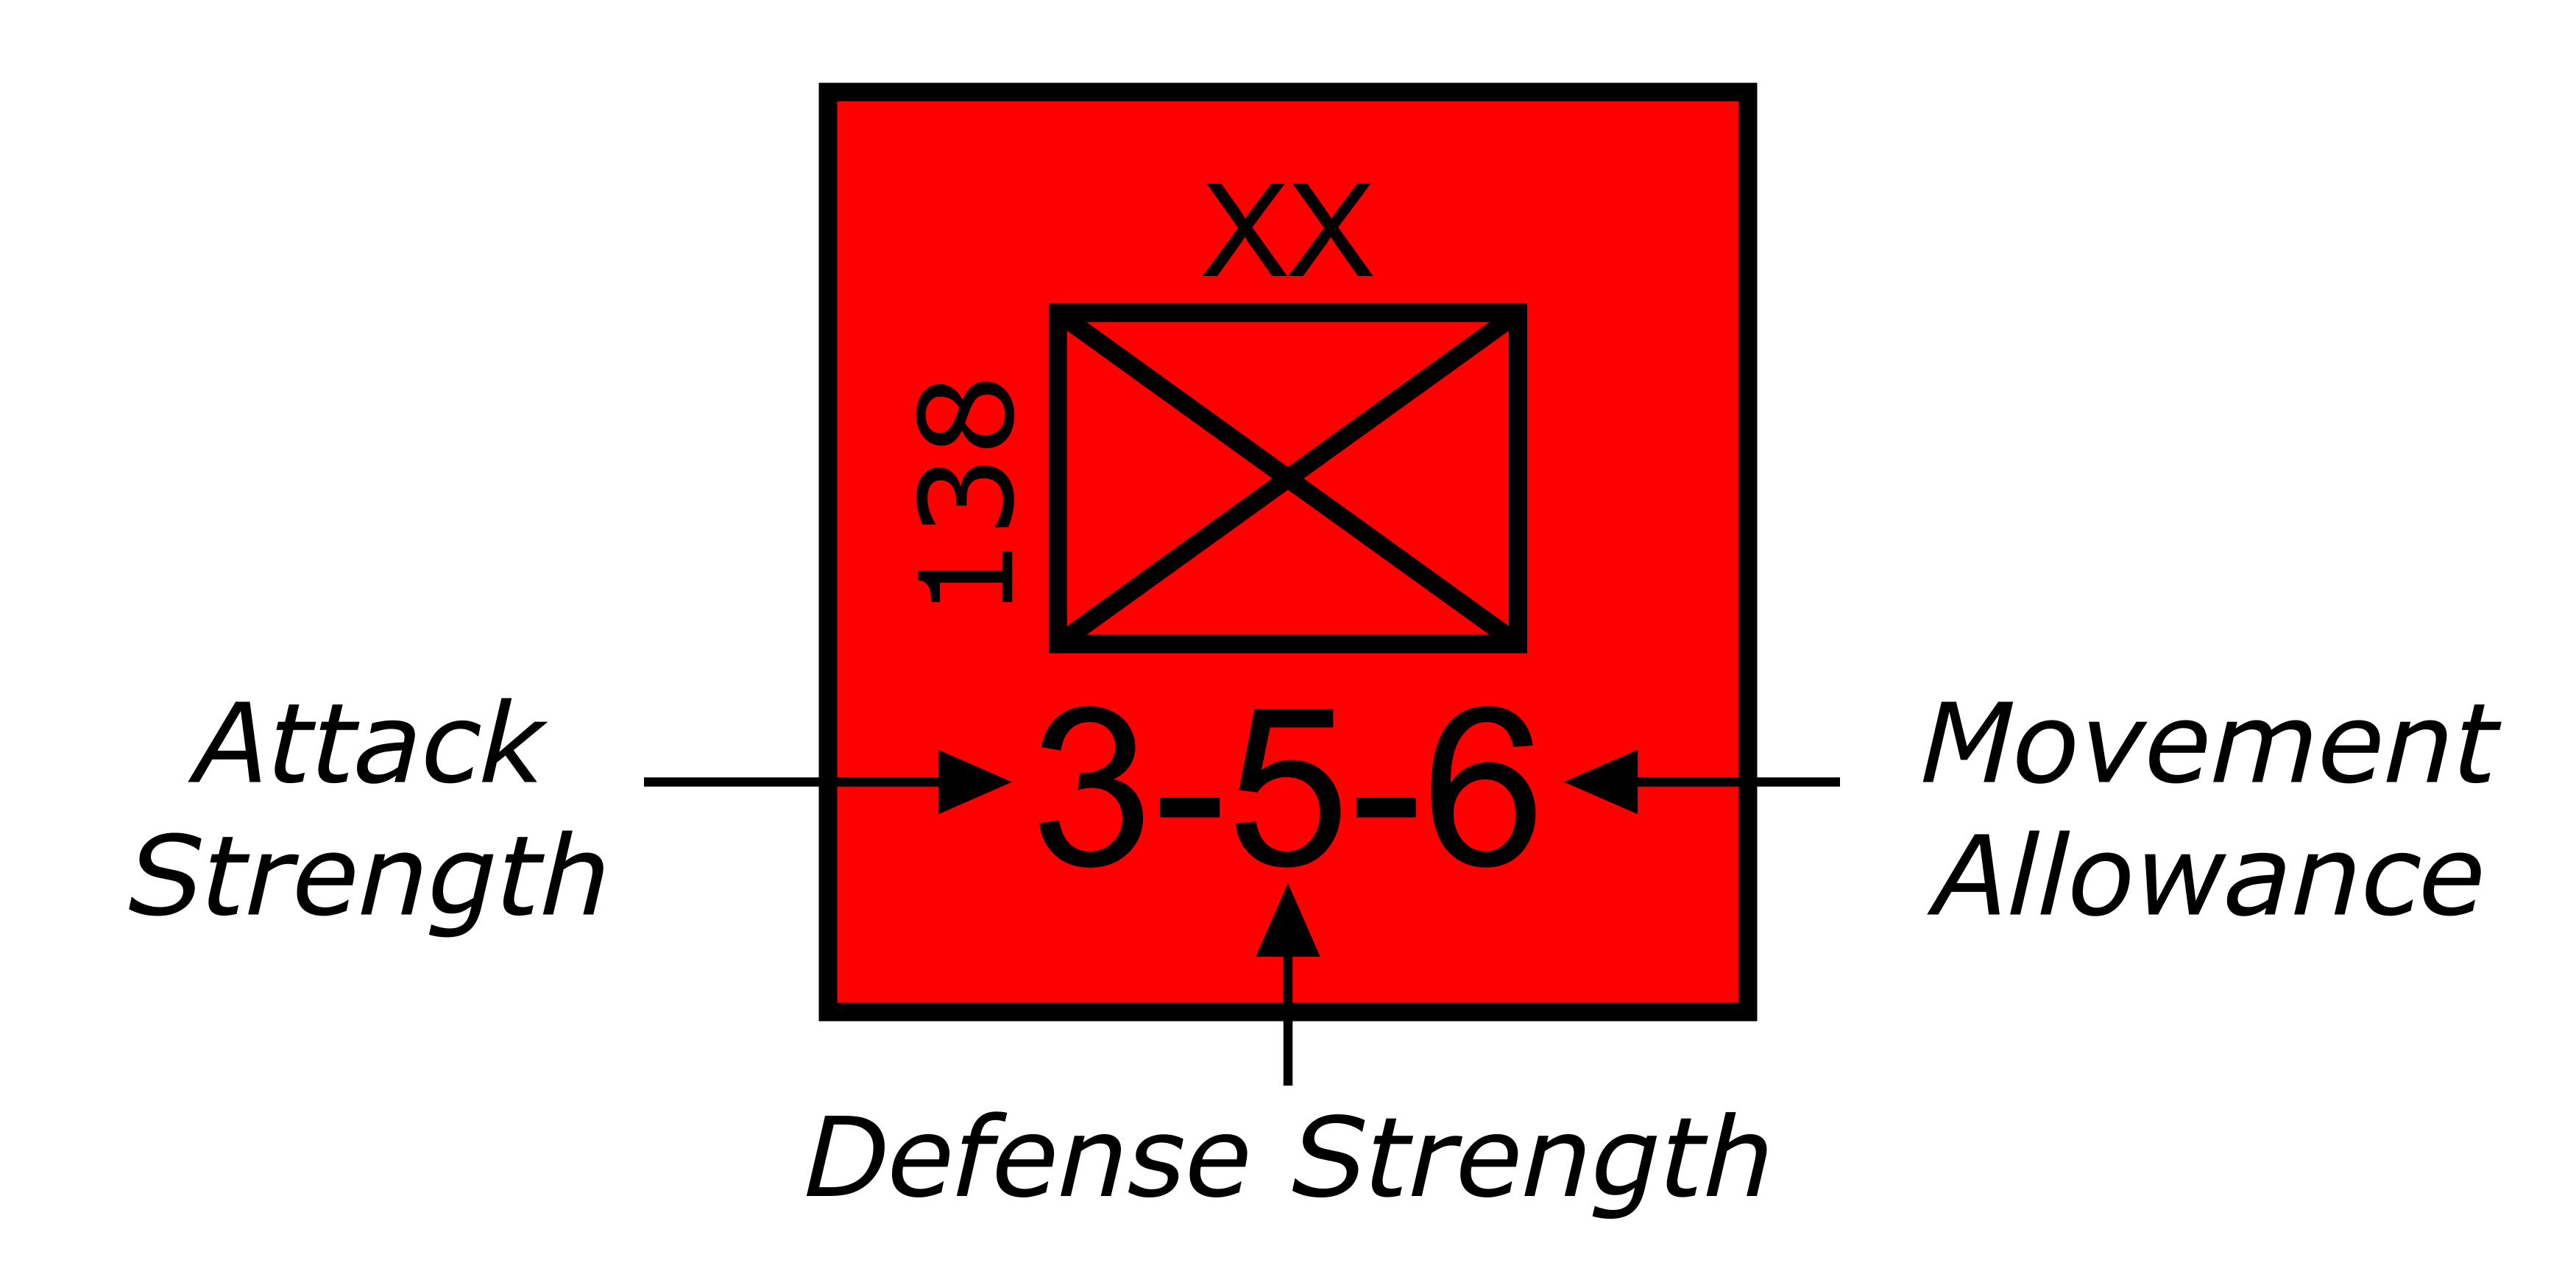
\includegraphics[scale=0.7]{soviet_unit_explained.png}
\end{center}

SOVIET UNIT (UNTRIED)

\begin{center}
  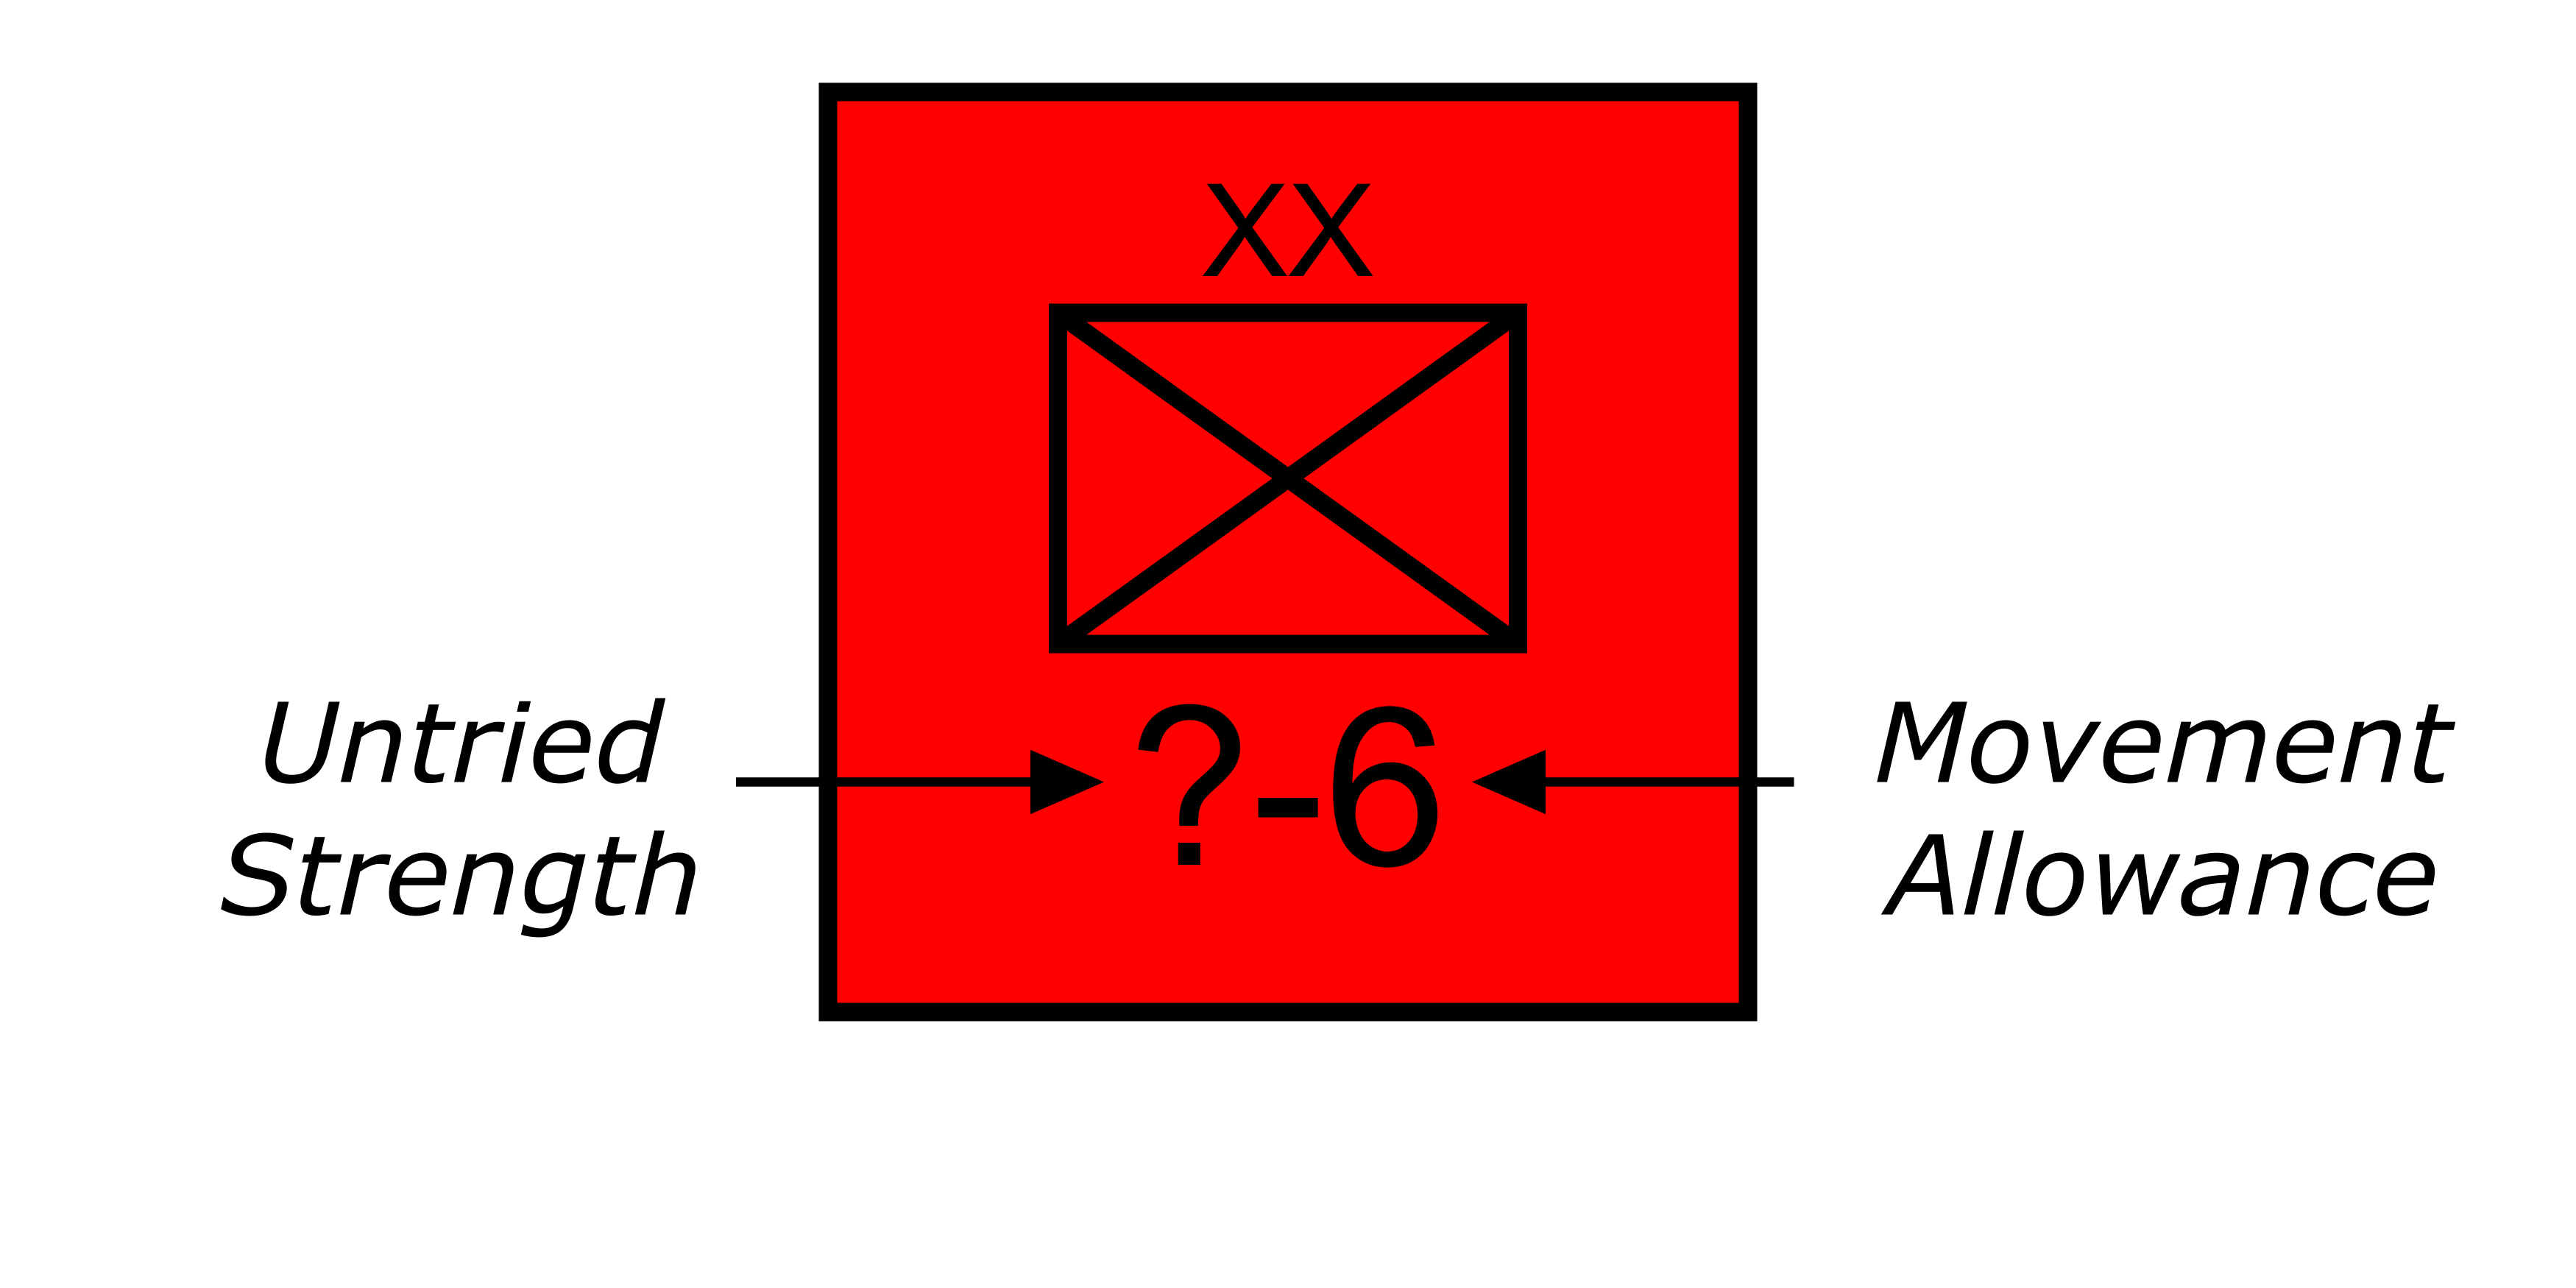
\includegraphics[scale=0.7]{soviet_unit_untried_explained.png}
\end{center}

SOVIET LEADER

\begin{center}
  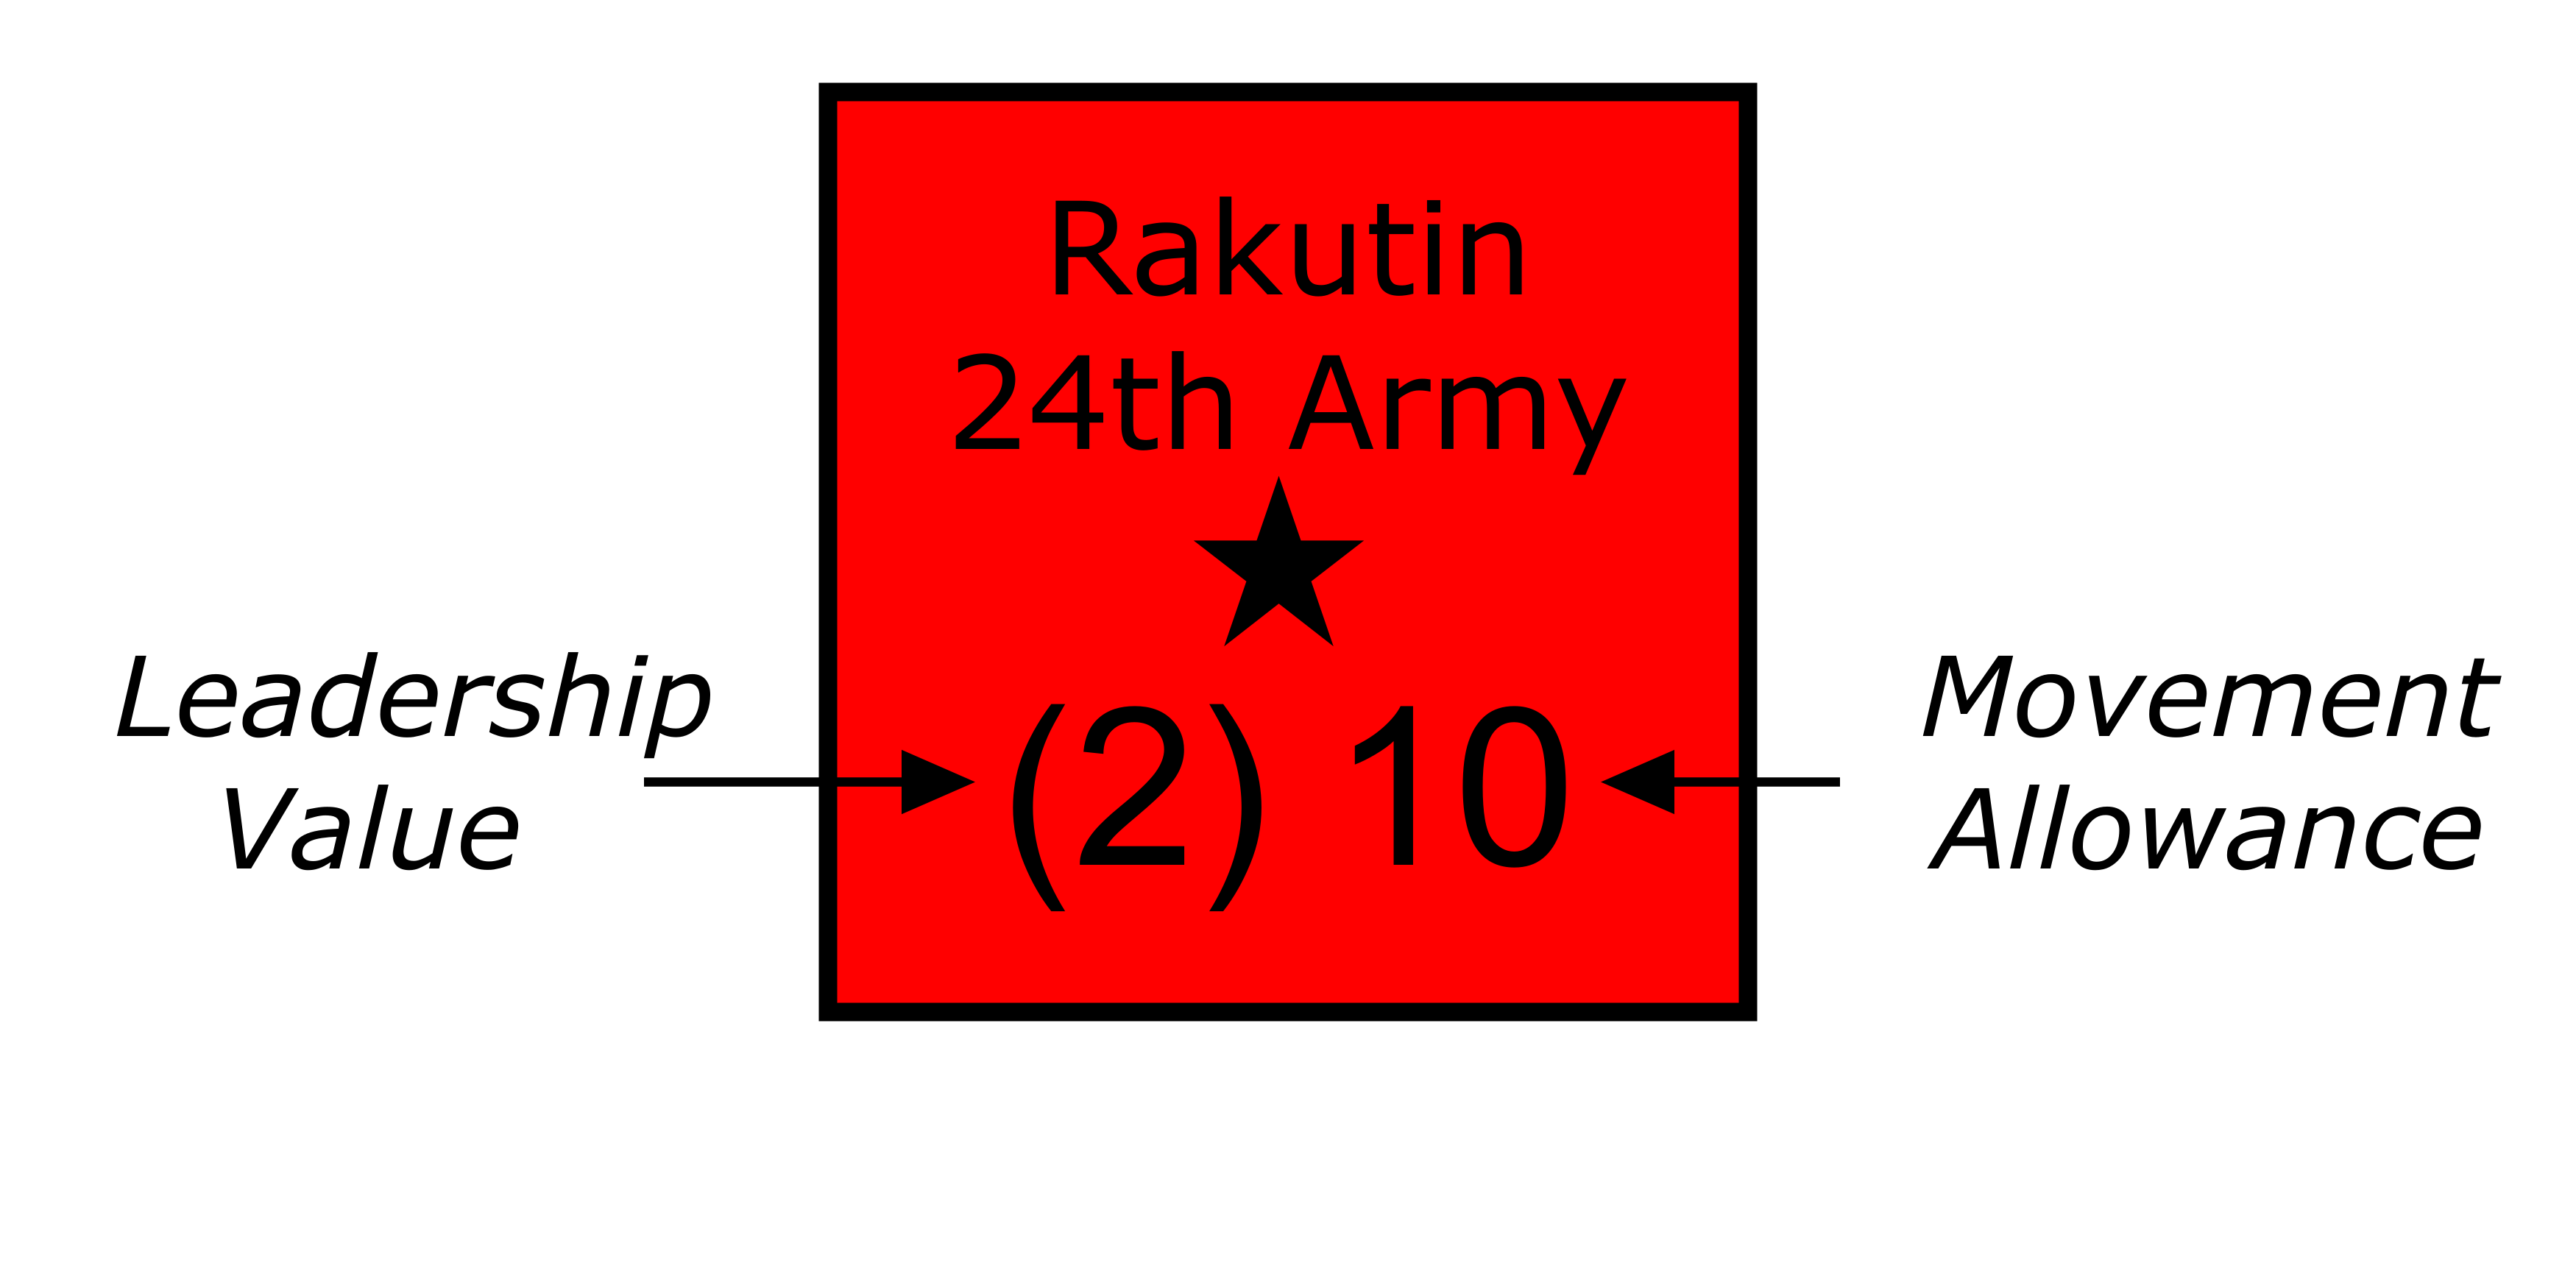
\includegraphics[scale=0.7]{soviet_leader_explained.png}
\end{center}

\textbf{Unit Designations}
These are the actual identity numbers of the units; divisions have but one number, while regiments have both their regimental identity and the number of the division of which they are a part (the number to the right of the slash is the division I.D.). For example, 20/12 indicates the 20th Panzer Regiment, which was part of the 12th Panzer Division.

\textbf{Unit Types}


\makebox[0.5\textwidth]{
  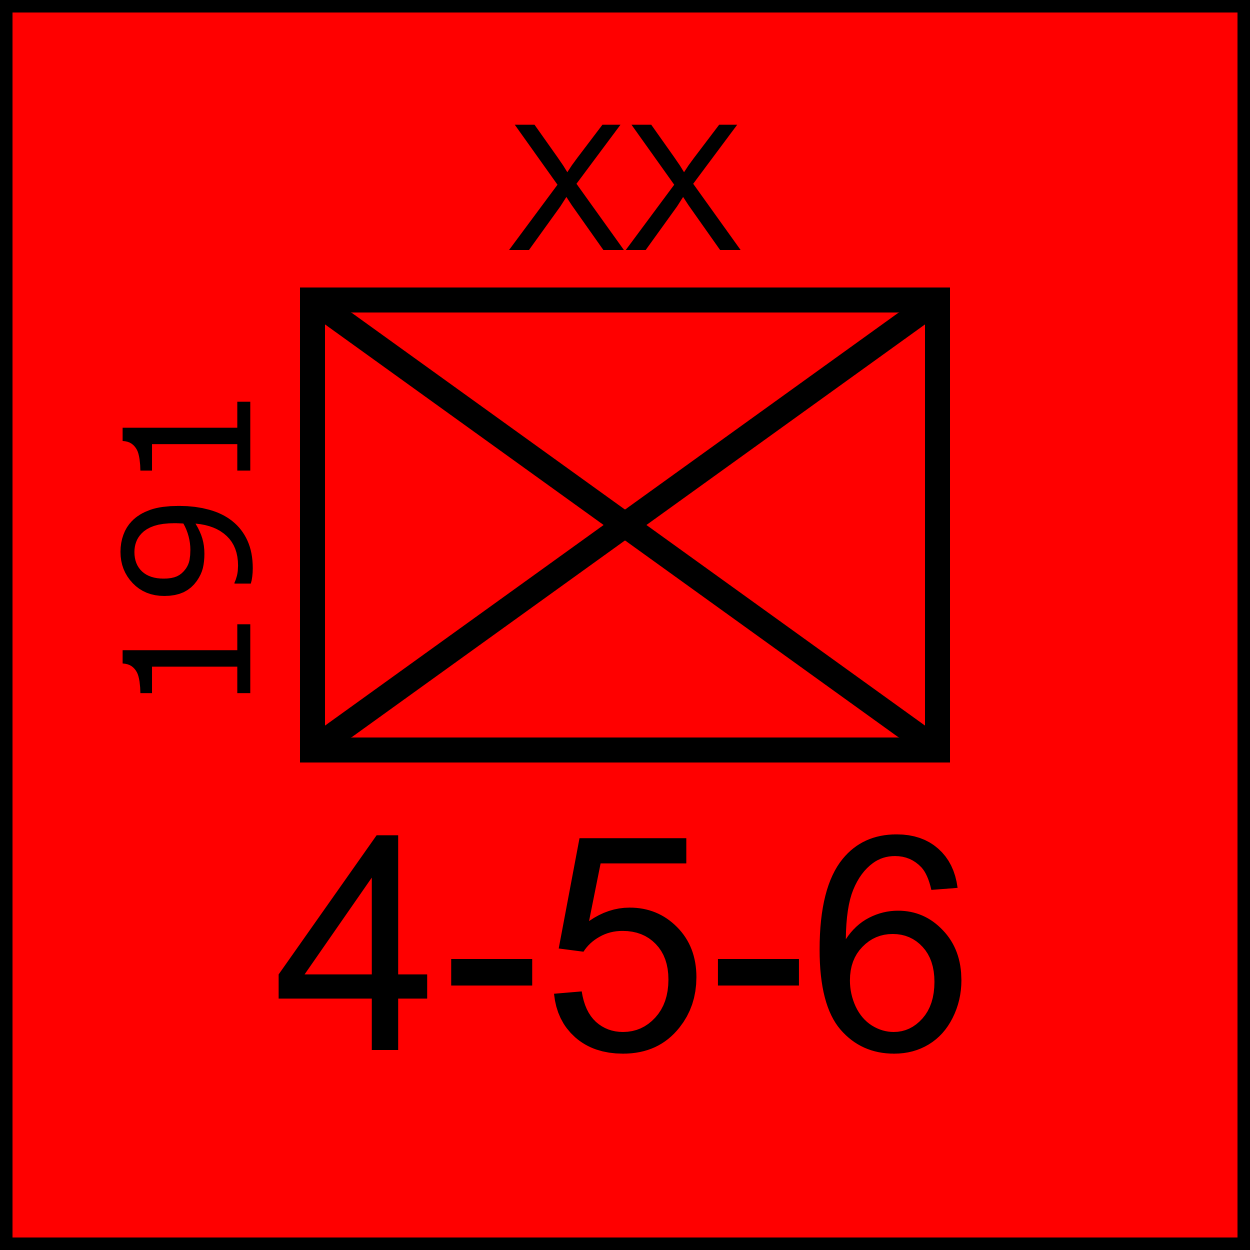
\includegraphics[scale=0.5]{soviet_infantry_unit_type.png}
  \raisebox{2.5em}{Soviet Infantry}
  \raisebox{0.5em}{Infantry (Motorized)}
  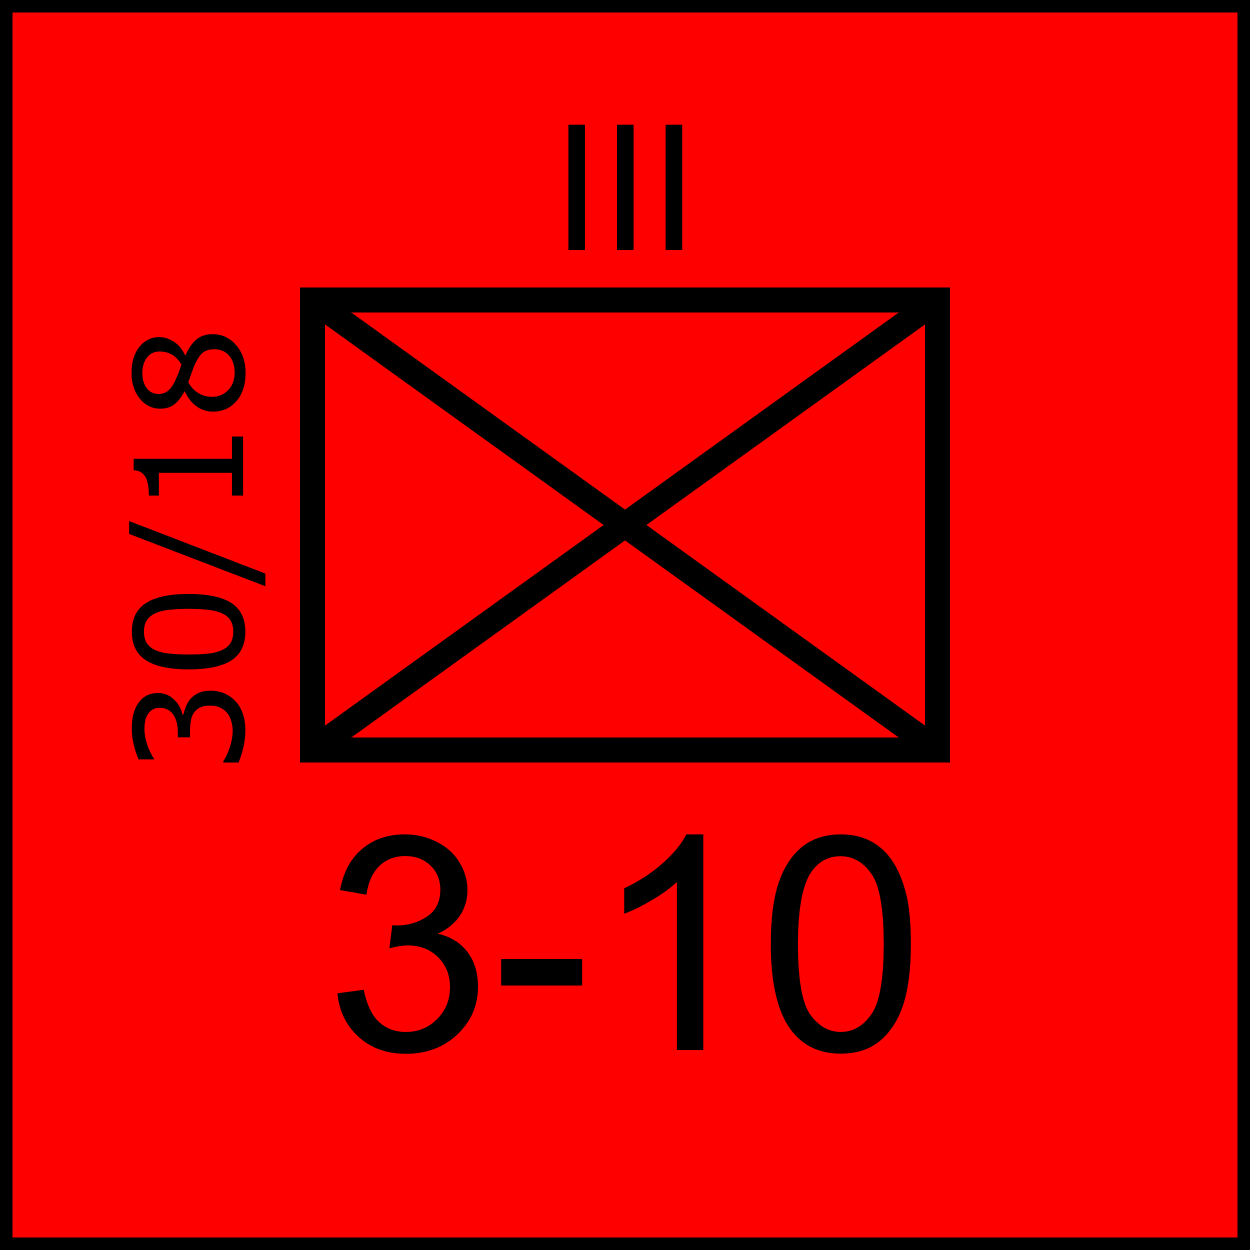
\includegraphics[scale=0.5]{soviet_motorized_infantry_unit_type.png}
}

\makebox[0.5\textwidth]{
  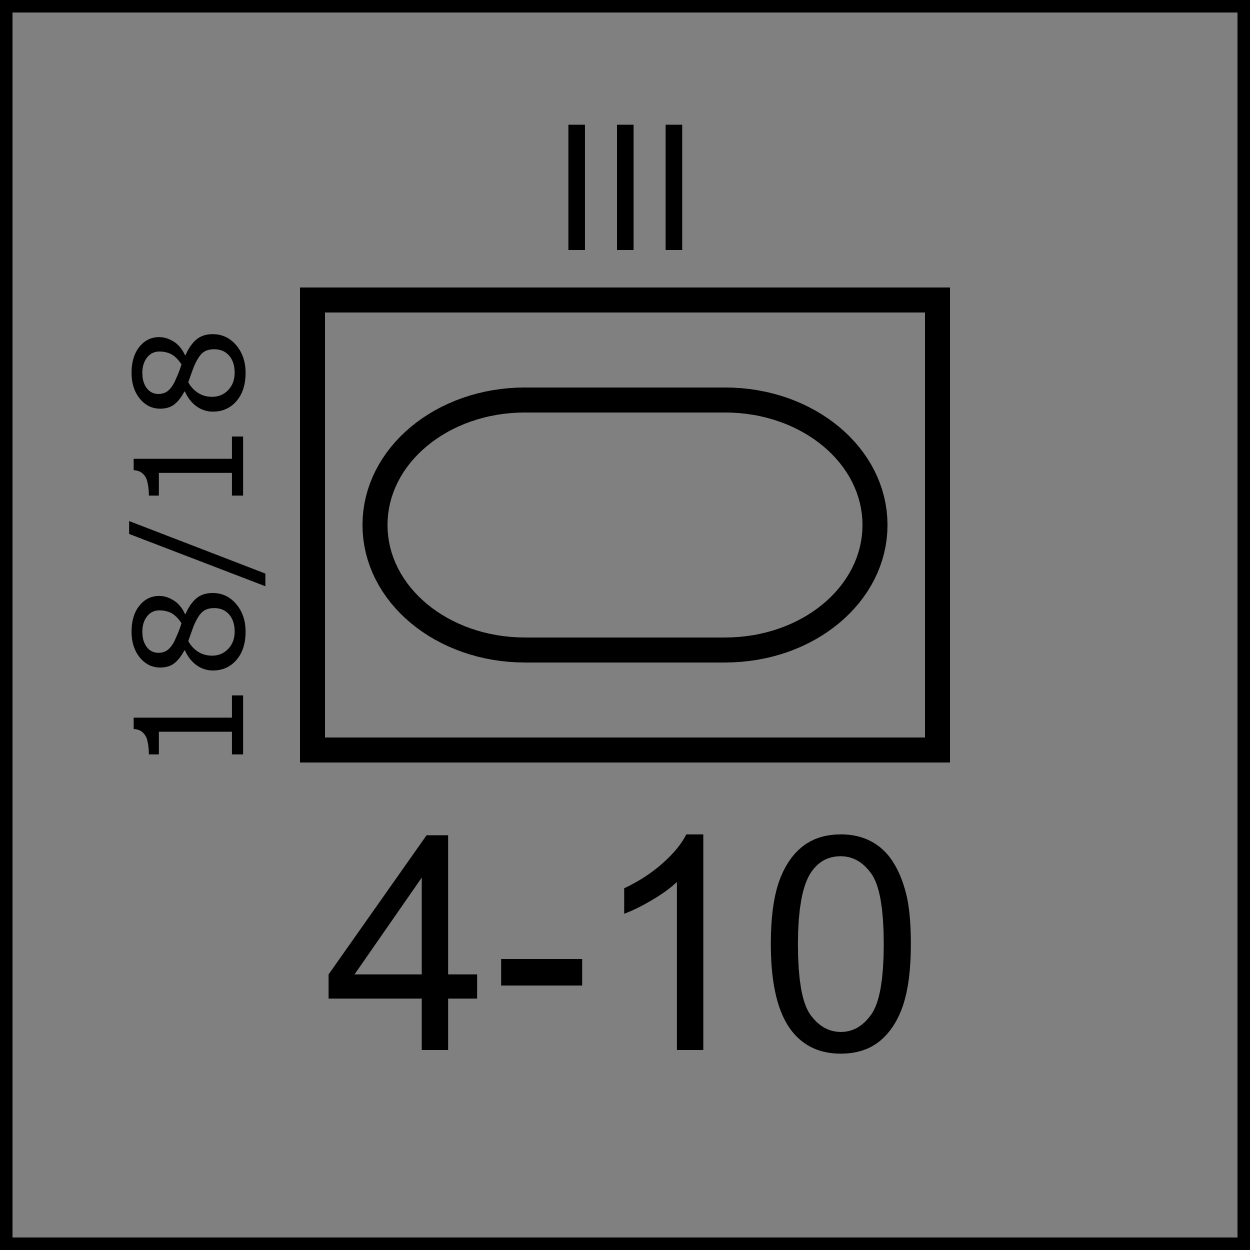
\includegraphics[scale=0.5]{german_armor_unit_type.png}
  \raisebox{2.5em}{Armor (Panzer)}
  \hspace{3em}
  \raisebox{1.5em}{Mechanized}
  \linebreak
  \hspace{-9em}
  \raisebox{0.5em}{(Panzer Grenadier)}
  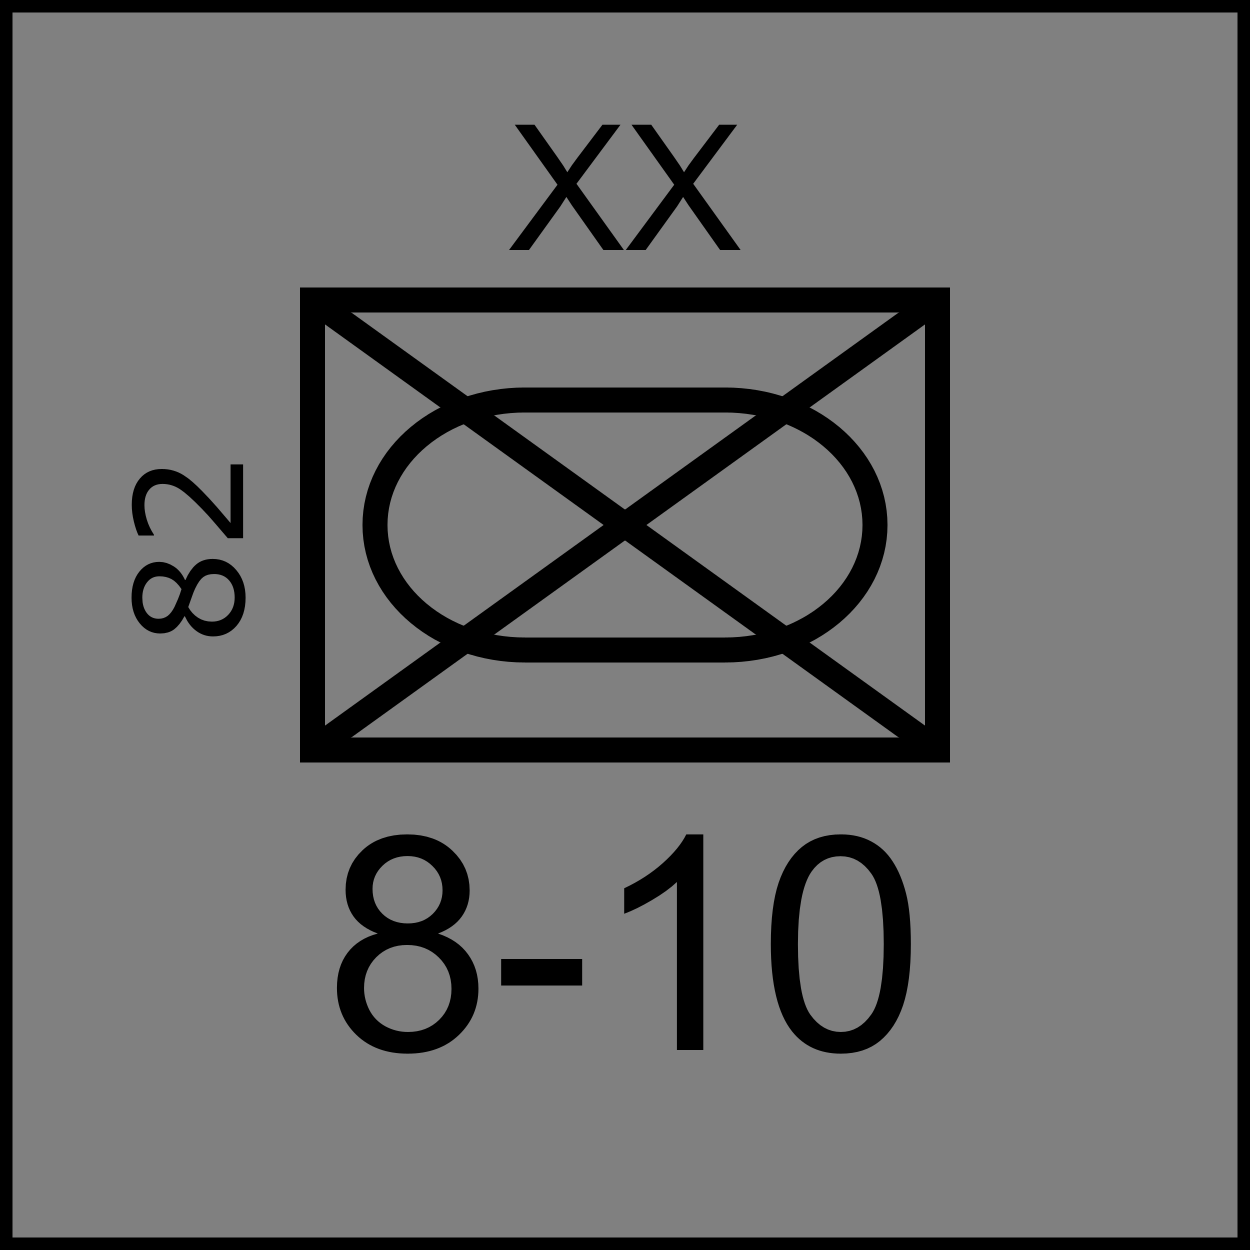
\includegraphics[scale=0.5]{german_mechanized_unit_type.png}
}

\makebox[0.5\textwidth]{
  
\includegraphics[scale=0.5]{air_interdiction_marker.png}
  \raisebox{2.5em}{Air Interdiction Marker}
  \hspace{-3.1em}
  \raisebox{0.5em}{Disruption Marker}
  
\includegraphics[scale=0.5]{disruption_marker.png}
}

\makebox[0.5\textwidth]{
  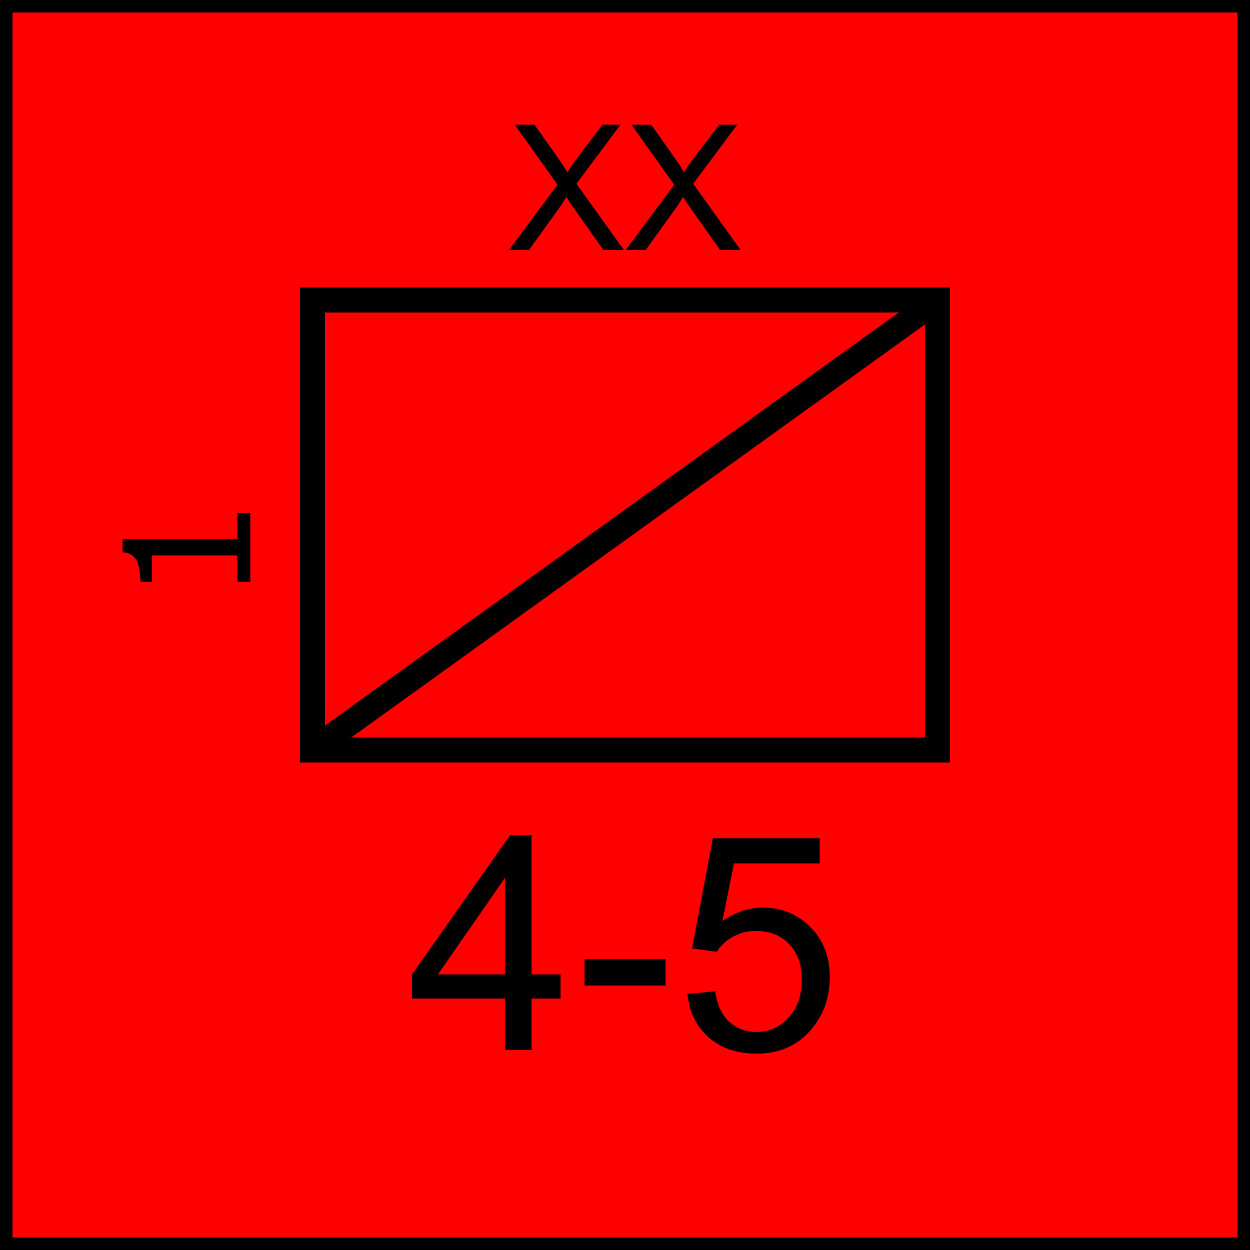
\includegraphics[scale=0.5]{soviet_cavalry.png}
  \raisebox{2.5em}{Cavalry}
  \hspace{4.5em}
  \raisebox{0.5em}{German Infantry}
  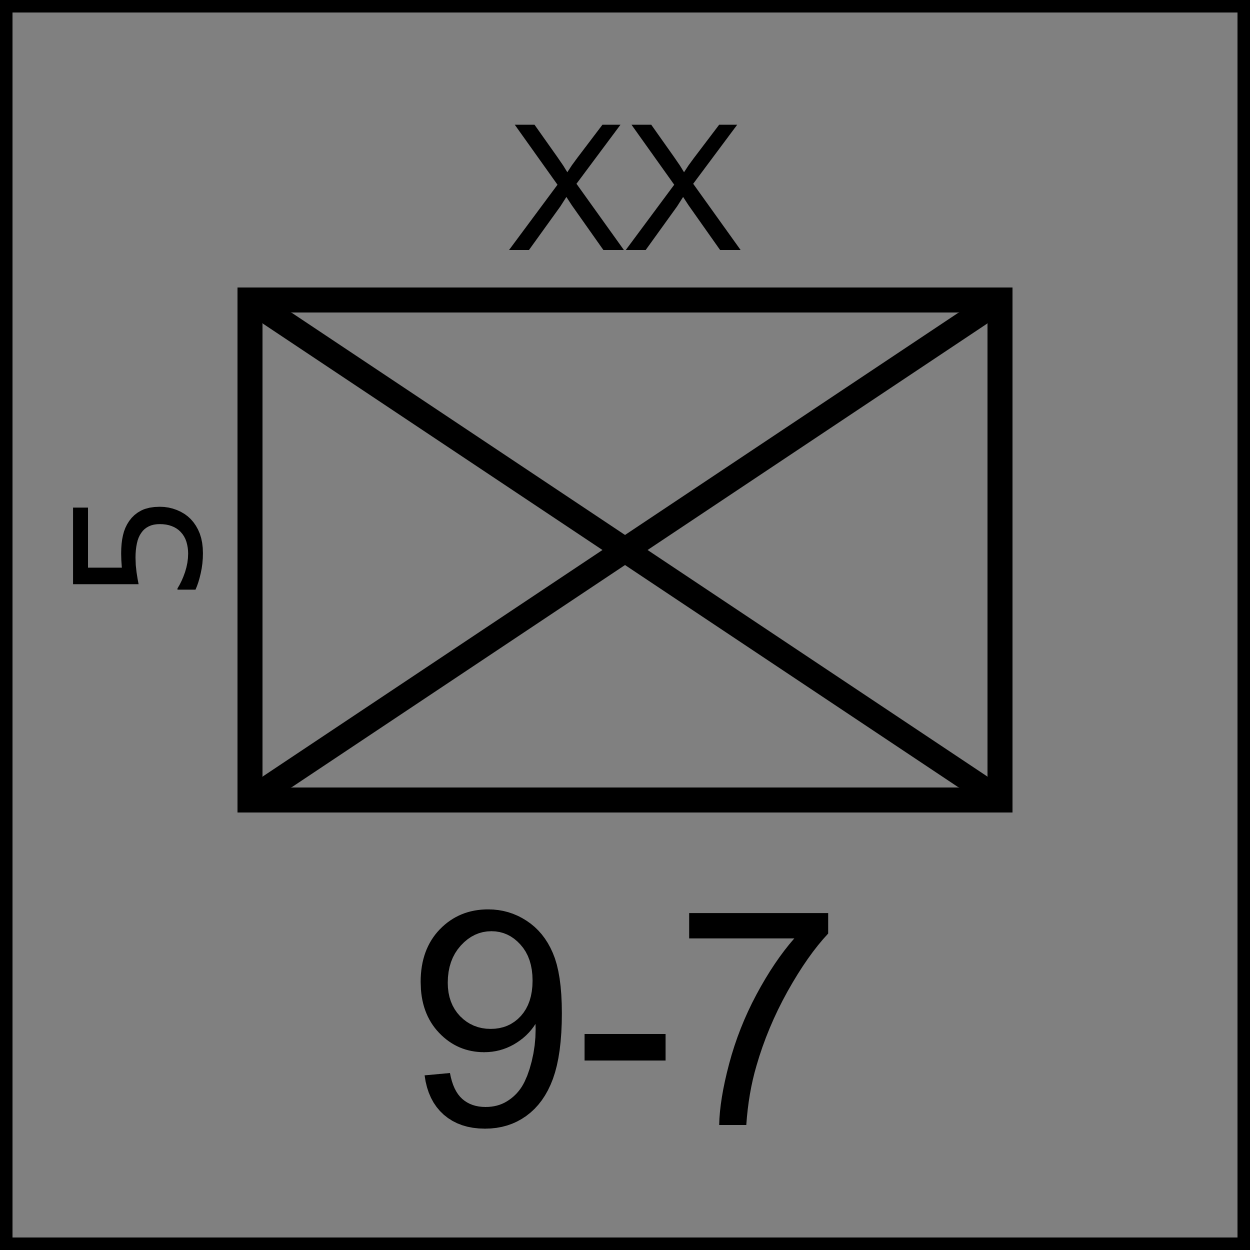
\includegraphics[scale=0.5]{german_infantry.png}
}

\textbf{Unit Sizes}
III=Regiment; XX=Division.

\textbf{Attack Strength} is the relative strength of a unit when attacking, expressed in terms of Strength Points.

\textbf{Defense Strength} is the relative strength of a unit when defending.

\textbf{Combat Strength} is the relative strength of a unit when attacking or defending.

\textbf{Untried Strength}, represented by a question mark; the true strength of the unit is revealed to both Players only after that unit has participated in combat.

\textbf{Leadership Value} is the rating of a particular leader, expressed in Leadership Points.

\subsection{PARTS INVENTORY}

The complete game of \textbf{Panzergruppe Guderian} should include the following parts:

\begin{itemize}
  \setlength\itemsep{-0.9em}
  \item 22"x32" Game Map
  \item Rules Folder
  \item Sheet of 200 Die-Cut Counters (some blank)
  \item Game Box (boxed version only)
  \item Plastic Die (boxed version only)
\end{itemize}

If any parts are missing or damaged, please write:
Customer Service
Simulations Publications, Inc.
44 East 23rd Street
New York, N.Y. 10010

Questions regarding the rules of the game will be answered if accompanied by a stamped, self-addressed envelope and if phrased to be answered by a simple one word answer. Send rules questions to the above address and mark the envelope "Rules Questions: Panzergruppe Guderian".\footnote{Included for completeness only. SPI is long gone.}
  \section{SEQUENCE OF PLAY}

\subsection{THE GAME-TURN}

\textbf{Panzergruppe Guderian} is played in Game-Turns; there are twelve Game-Turns in a complete game. Each Game-Turn is composed of two Player-Turns. The Player whose Player-Turn is in progress is called the Phasing Player. Each Game-Turn proceeds strictly as follows.

\begin{flushleft}
  \subsection{GAME-TURN SEQUENCE OUTLINE}
\end{flushleft}

A. SOVIET PLAYER TURN

\textbf{1. Movement Phase:} The Soviet Player checks for Supply; he then moves any or all of his units in any direction or directions, to the limit of each unit's Movement Allowance, and within the restrictions outlined in the Rules of Movement and Supply. The Soviet Player may conduct Overruns in this Phase. He also brings in his Reinforcements according to the Reinforcement Schedule. At the end of this Phase, German Air Interdiction Markers are removed.

\textbf{2. Combat Phase:} Soviet units may attack German units according to the Rules of Combat.

\textbf{3. Disruption Removal Phase:} The Soviet Player may remove all Disruption Makrers from units that have suffered Disruption as a result of Overrun.

\textbf{4. Soviet Interdiction Phase:} The Soviet Player may choose this Turn as one of the three Turns in the game in which he may use Interdiction. If he does, he places his Interdiction Marker on the game map according to the Rules for Soviet Interdiction.

B. GERMAN PLAYER TURN

\textbf{1. Initial Movement Phase:} The German Player checks for Supply. He may then move his units, bring in reinforcements, and conduct Overruns.

\textbf{2. Combat Phase:} German units may attack Soviet units.

\textbf{3. Mechanized Removal Phase:} German Panzer, Mech, Motorized and Cavalry units may move again, if possible. German units may conduct Overruns in this Phase.

\textbf{4. Disruption Removal Phase:} The German Player removes any Disruption Markers from his units.

\textbf{5. Air Interdicition Phase:} The German Player may place his Air Interdiction Markers on the game map according to the rules for Air Interdiction. He may remove any Soviet Interdiction Markers on the game map.

C. GAME-TURN INDICATION

AFter both Players have completed their respective Player-Turns, the Game-Turn is completed. The Game-Turn Marker is advanced on the Game-Turn Record Track, signalling the start of a new Game-Turn.
  \section{INITIAL SET-UP}
GENERAL RULE:
The Soviet Player places his initial units on the map first, in accordance with the placement listed below. After the Soviet Player has placed all his initial units, the German Player places his three Air Interdiction Markers in accordance with Case 12.2. The game then begins.

The Soviet Player always moves first in each Game-Turn. Note that there are no German units (except for Interdiction Markers) on the game map during the Soviet Player-Turn. German Air Interdiction Markers are placed on the map before the die roll specified in Case 5.21 is attempted.

Punch out all Soviet combat units, and turn them face-down so that their Untried side is showing. The Soviet Player now randomly chooses the number of units specified, making certain to choose the type called for. All the units are then stacked in the hex listed. Stacking restrictions must not be exceeded at the end of the First Soviet Movement Phase. If more than one hex is listed, the Soviet units may be placed in any of the hexes, within stacking restrictions (see Case 12.1).

\subsection{SOVIET INITIAL DEPLOYMENT}
\textbf{In hex 4015}:
The 24th Army (5 Rifle Divisions, 1 Armored Division, General \textbf{Rakutin}).

\textbf{In hex 2216}:
The 16th Army (6 Rifle Divisions, General \textbf{Lukin}).

\textbf{In hex 1414}:
The 19th Army (4 Rifle Divisions, General \textbf{Konlev}).

\textbf{In hex 0123, 0124, 0125 and/or 0126:}
The 13th Army (7 Rifle Divisions, 1 Armored Division, General \textbf{Remezov}).

\textbf{In hexes 0108, 0109, 0110, 0111, 0112, 0113, 0114, and/or 0115:}
The 20th Army (6 Rifle Divisions, 4 Armored Divisions, General \textbf{Kurochkin}).

\subsection{SOVIET FIRST TURN SPECIAL RULES}

The Soviet Player is somewhat restricted as to what he may do on his First Player-Turn.

\subsubsection{} The die must be rolled once for each Army to determine whether the 16th Army (2216) and the 19th Army (1414) may be moved on Turn One. If the Soviet Player rolls a "1", "2" or "3", the army in question may move. Any number other than those given results in that army standing in place for the entire Turn (see Case 5.22). Both armies are free to move on Game-Turn Two.

\subsubsection{} If the 16th and/or the 19th Army is unable to move, it must still satisfy stacking restrictions by the end of the Movement Phase. To do so, the Player may, if necessary, move as many units as are needed one hex (maximum) to satisfy the stacking restrictions.

\subsubsection{} All units of the 13th and 20th Armies \textbf{must expend their full Movement Allowance in the First Game-Turn}. They may not end the Movement Phase of the First Game-Turn in either of the two westernmost hexrows (0100 and 0200) on the game map, nor may they enter any hex more than once. Moreover, they may never move in a westerly direction; they may move north, south, or east only. Neither the 13th nor the 20th Army may use Rail Movement on the First Game-Turn.
  \section{MOVEMENT}

GENERAL RULE:

During the Movement Phase, the Phasing Player may move as many or as few of his units as he wishes. During his Friendly Movement Phase (and for mechanized units, again during the German Mechanized Movement Phase), each unit may move as many or as few hexes as desired as long as its Movement Allowance is not exceeded in a \textbf{single} Movement Phase. Unused Movement Points may not be accumulated or transferred.

PROCEDURE:

Move each unit individually, tracing the path of its movement through the hexagonal grid. Once the Player's hand is removed from the unit, movement is considered completed.

CASES:

\subsection{HOW TO MOVE UNITS}

\subsubsection{} During a Movement Phase, all, some or none of a Player's units may be moved. No other units may be moved. Combat may not occur in this Phase; however, \textbf{Overrun} - a form of combined combat and movement - may take place in this Phase. See Case 6.5.

\subsubsection{} Movement is calculated in terms of Movement Points. Basically, each unit expends one Movement Point of its total Movement Allowance for each Clear terrain hex it enters; other terrain costs \textbf{more} than one Movement Point to enter or cross. These effects are summarized on the Terrain Effects Chart (6.7).

\subsection{MOVEMENT INHIBITIONS AND PROHIBITIONS}

\subsubsection{} A Friendly unit may never enter a hex containing an Enemy unit.

\subsubsection{} A unit must stop upon entering an Enemy-controlled hex (see Section 8.0); Once a unit is in an Enemy Zone of Control, it may not leave that hex voluntarily.

\subsubsection{} A unit may not expend more Movement Points that its total Movement Allowance in any \textbf{one} Movement Phase. (Note that German mechanized units have \textbf{two} Movement Phases and may expend their full Movement Allowance in \textbf{each} phase). A unit may use all, some or none of its Movement Points in a given Phase. However, a unit may not "save" Movement Points for another Turn, nor may unused Points be transferred to another unit.

\subsubsection{} Units may move only during their Friendly movement Phase(s), although there may be some movement as a result of combat, in terms of advances and retreats. These are not considered to be "movement" and do not require the expenditure of Movement Points.

\subsubsection{} Units that are out of supply (Section 11.0) have their Movement Allowance halved, dropping all fractions.

\subsection{RAIL MOVEMENT}

\subsubsection{} The Soviet Player - and only the Soviet Player - may move up to eight combat units, plus any number of Leaders, by Rail each Turn. For the purposes of Rail Movement, each Soviet division tank or mechanized counts as \textbf{three} combat units.

\subsubsection{} In order to move by Rail, a unit must start the Movement Phase \textbf{in a} Railroad hex and it must finish that Phase on a Railroad hex. It must move from Rail hex to adjacent, connected Rail hex only in that Phase. The units may not enter an Enemy Zone of Control when travelling by Rail. Units entering the game as reinforcements may use Rail Movement if they enter the game map on a Railroad hex. Reinforcements using Rail Movement \textbf{do} count against the eight combat unit maximum. (Remember, Leaders do not count).

\subsubsection{} Soviet units using Rail Movement may move \textbf{thirty} hexes by Rail in any one Turn. German Air Interdiction may limit movement by Rail by increasing the cost per Rail hex (see Section 12.0). Terrain has no effect on Rail Movement.

\subsubsection{} Units do not have to be in supply to use the \textbf{full} Railroad Movement bonus, nor do they have to be within a Leader's radius (see Case 10.21).

\subsubsection{} Aside from providing the Soviets with added movement capabilities, the Railroads have no other function in the game. They affect neither supply nor normal movement.

\subsubsection{} German units may not use Rail Movement.

\subsection{SPECIAL SOVIET MOVEMENT RESTRICTIONS}

For the first \textbf{six} Game-Turns, no Soviet unit (with the exception of the units noted in Case 5.23) may enter, voluntarily or involuntarily, the first two hexrows of the western edge of the game map (0100 and 0200). Soviet units may \textbf{attack} German units that are in these hexrows, but they may not advance after combat. Soviet Units may not attempt to \textbf{Overrun} German units in these hexrows. If forced to retreat into one of these hexrows, a Soviet unit is eliminated. However, Soviet units may trace Supply Lines and Leadership Radii through these hexrows.

\subsection{OVERRUN}

During a Movement Phase - and \textbf{only} during a Movement Phase - the Phasing Player may attempt to Overrun any Enemy unit. For game purposes, Overrun is considered to be a function of movement. Both sides may conduct Overruns in their respective Movement Phases; the Germans, having two Movement Phases, may conduct Overruns in both Movement Phases.

\subsubsection{} To conduct an Overrun, the Phasing Player, in a Friendly Movement Phase, moves his unit(s) adjacent to the target hex. All of the units which participate in the Overrun must be in the same hex. The Phasing units, if they wish to Overrun, must then expend three additional Movement Points to attack \textbf{all} Enemy units in the target hex. The Phasing units' Attack Strengths are reduced by half, dropping fractions. All terrain rules and Supply rules are in effect. If, as a result of the Overrun, the Enemy hex is vacated, the Friendly, Overrunning Player \textbf{must} then move all of the attacking units into the vacated hex (however, see Case 6.52). There is no cost for moving into the vacated hex. The victorious Overrunning units may then if they so desire, continue normal movement if they have any remaining Movement Points and they are not \textbf{then} in an Enemy Zone of Control. The Phasing units may conduct further Overruns if they have the necessary Movement Points.

\subsubsection{} If an Overrun attack fails to dislodge the Enemy units from the hex, the Overrunning units may not move any further in that Movement Phase. Overrunning units do \textbf{not} move into a vacated target hex if the combat result is a "split" result (see Case 9.67) or an "engaged" result (see Case 9.68). In addition, a "split" or "engaged" result stops movement for the affected units for the remainder of that Phase. Any combat result where the attacker/Overrunning unit must take a loss or retreat halts movement for that Phase.

\subsubsection{} Soviet Leaders may be Overrun like any other units. However, Soviet Leaders may \textbf{not} conduct Overruns by themselves as they have no Attack Strength (see Cases 10.22 and 10.36).

\subsubsection{} All units conducting an Overrun against an individual target hex \textbf{must} start the Movement Phase in the same hex. Individual Overruns may be conducted against more than one unit, but all these units must be in the same hex. Individual Overruns may be conducted against more than one unit, but all these units must be in the same hex. You may not attempt to Overrun more than one hex at any one time, although you may conceivably conduct more than one Overrun in a given Movement Phase. A defending unit may conceivably be Overrun by different unit more than once in a Phase.

\subsubsection{} A unit conducting an Overrun attacks at \textbf{half} Strength. The halving is done after all adjustments to the Combat Strength have been made. All fractions remaining after this final adjustment are then dropped. Thus, a German Panzer Division (worth eight Combat Strength Points at face value) that is out of supply and conducting an Overrun would Overrun with a Strength of four. (Its total Strength would be doubled for divisional integration, see Case 7.3, halved for being out of supply and then halved again for Overrun). Note that Soviet units that begin a Friendly Movement Phase beyond the Radius of a Leader may \textbf{not} conduct Overruns.

\subsubsection{} When conducting an Overrun attack, Players may ignore the Zones of Control of units which are exterting influence on the hex from which the Overrun attack is coming. That is, they may occupy the target hex if the Overrun is successful regardless of other Enemy ZOC's. However, if the Friendly unit finishes an Overrun in an Enemy Zone of Control, it may not \textbf{move} any further in that Movement Phase; however, it may conduct another Overrun on an adjacent hex providing it has the necessary Movement Points.

\subsubsection{} Units conducting Overruns may \textbf{not} conduct "advance after combat" (see Case 9.7); they can move into the vacated target hex, but may not move further without expending Movement Points. Remember, Overrun is movement, not combat.

\subsubsection{} Enemy units that \textbf{defend} successfully against an Overrun attack to not move into a vacated hex or advance after combat. They remain in their hex.

\subsection{DISRUPTION}

\subsubsection{} Units that are \textbf{defending} against an Overrun and suffer any loss or retreat (not including an Engaged) as a result of the Overrun are considered to be \textbf{Disrupted}. Only defending units can become Disrupted and Disruption pertains only to a Overrun - not normal combat. The status of Disruption is indicated by placing a Disrupted Marker on top of the unit(s).

\subsubsection{} Disrupted units may not attack; they do defend normally. They may \textbf{not} move, nor do they exert a Zone of Control. Additional "Disruption" results and/or normal combat results have not further Disruption effect.

\subsubsection{} Disrupted units return automatically to normal in the applicable Friendly Disruption Removal Phase.

\subsubsection{} If a Soviet Leader becomes Disrupted it may not function as a Leader, although it continues to function as a normal - if Disrupted - combat unit. Disrupted Soviet Leaders may not coordinate supply and/or combat for regular Soviet combat units, nor may they aid Soviet attacks.

\subsection{TERRAIN EFFECTS CHART}

  \section{STACKING}

\subsection{SOVIET RESTRICTIONS}

The Soviet Player may never have more than three \textbf{combat} units in any one hex at the end of his Movement Phase and at \textbf{any} time during the Combat Phase. He may have as many as four units of \textbf{any} kind in a hex, as long as at least one of the units is a Leader. Informational Markers, such as German Air Interdiction Markers and Disrupted Markers, never count against stacking. Units may pass freely through other stacks of Friendly units, except during retreats, and the restrictions of stacking apply only at the end of the Friendly Movement Phase and throughout all Combat Phases. If units are found to be in excess of the stacking restrictions at the end of a Friendly Movement Phase or any Combat Phase, the excess must be eliminated and removed from the game, at the choice of the Owning Player.

\subsection{GERMAN RESTRICTIONS}

The German Player may never have more than three combat units in any one hex at the end of either of his Movement Phases or at the end of any Combat Phase. The same penalties for overstacking as apply to the Soviets (7.1) apply to the Germans.

\subsection{GERMAN DIVISIONAL INTEGRATION}

If the German Panzer, Mech, or Motorized units in a hex comprise \textbf{all} the units of a division, the total Strength of the units in that hex is doubled for both attack and defense. There may not be any units from any other division in that hex, and \textbf{all} units from the division must be in the hex. Each Panzer Division has one Panzer and two Panzer Grenadier regiments, and each Motorized Infantry Division has two regiments, with the exception of the \textbf{Das Reich} Motorized Infantry Division, which has three regiments. German Infantry and Cavalry Divisions do not qualify for this combat bonus. If any regiment in a division is eliminated, the combat bonus may not be used by that division.
  \section{ZONES OF CONTROL}

GENERAL RULE:

The six hexagons surrounding a hex constitute the Zone of Control (ZOC) of any units in that hex. Hexes upon which a unit exerts a Zone of Control are called controlled hexes, and inhibit the movement of Enemy units. All units must cease movement when they enter an Enemy-controlled hex and may not leave that hex voluntarily.

CASES:

\subsection{EFFECTIVENESS OF\\*ZONES OF CONTROL}

\subsubsection{} All units exert a Zone of Control at all times during the entire Game-Turn,unless they are in a state of Disruption. Disrupted units have no ZOC.

\subsubsection{} Units never pay any additional cost to enter an Enemy-controlled hex.

\subsubsection{} Units may never voluntarily leave an Enemy controlled hex. Friendly units may leave Enemy-controlled hexes only as a result of combat. However, see Overrun Rules in Case 6.5.

\subsubsection{} Friendly units (but \textbf{not} Friendly ZOC's) negate the presence of Enemy Zones of Control for the purposes of tracing Supply Lines and Leadership Radii. They do not negate Enemy Zones of Control for purposes of movement. They also negate the effect of an Enemy ZOC for the purposes of retreat.

\subsubsection{} If a given unit is in an Enemy-controlled hex, the Enemy unit is also in its Zone of Control. The two units are equally and jointly affected.

\subsubsection{} Zones of Control extend into all six hexes adjacent to the controlling unit's hex. Zones of Control extend across River hexsides; however, they do \textbf{not} extend across all-Lake hexsides. No other terrain affects Zones of Control.

There is no additional effect of having more than one unit exerting its Zone of Control onto a given hex.
  \clearpage
\section{COMBAT}

GENERAL RULE:

Combat occurs between adjacent opposing units at the Phasing Player's discretion. The Phasing Player is the attacker, the non-Phasing player is the defender, regardless of the overall strategic situation.

PROCEDURE:

Total the Attack Strengths of all the attacking units involved in a specific attack and compare it to the total Defense Strength of the units in the hex under attack. State the comparison as a probability ratio: Attacker's Strength to Defender's Strength. Round off the ratio in favor of the defender to conform to the simplified odds found on the Combat Results Table; roll the die and read the result on the appropriate line under the odds. Apply the result immediately, before resolving any other attacks being made during the Combat Phase.

CASES:

\subsection{WHICH UNITS MAY ATTACK}

\subsubsection{} Units may attack only during their own Friendly Combat Phase (see also Overrun, 6.5). They may then attack any and all Enemy units which are adjacent to them. Only those units directly adjacent to a given Enemy unit may participate in an attack upon that unit.

\subsubsection{} Attacking is completely voluntary; units are never compelled to attack, and not every unit adjacent to an Enemy unit need participate in any attack. A Friendly unit in a stack that is not participating in a given attack is never affected by the results of that attack.

\subsubsection{} An Enemy-occupied hex may be attacked by as many units as can be brought to bear in the six adjacent hexes.

\subsubsection{} No unit may attack more than once per Combat Phase and no Enemy unit may be attacked more than once per Combat Phase. [Remember, Overrun is \textbf{not} combat].

\subsection{MULTIPLE UNIT AND\\MULTI-HEX COMBAT}

\subsubsection{} All units in a given hex must be attacked as a single Defense Strength. The defender may not withhold a unit in a hex under attack. Different units in a hex may not be attacked separately, nor may one unit be attacked without involving the other units in the same combat.

\subsubsection{} Other units in a hex that contains an attacking unit need not participate in that same combat or any other attack. Thus when one unit in a stack is attacking a given hex, the other units in the stack could attack a different hex, or not attack at all.

\subsubsection{} If a unit(s) is adjacent to more than one Enemy-occupied hex, it could attack all of them in a single combat. Thus, units in a single hex may attack more than one hex. The only requirement is that all attacking units must be adjacent to all defending units.

\subsubsection{} A given unit's Attack and/or Defense Strength is always unitary; that is, it may not be divided among different combats either for attack or defense.

\begin{flushleft}
  \subsection{EFFECTS OF TERRAIN ON COMBAT}
\end{flushleft}

\subsubsection{} Units defending in certain types of terrain may have their Defense Strength increased. This is always expressed as a multiple of the Defense Strength. (A unit with a Defense Strength of four in a Major City defends with a Strength of eight).

\subsubsection{}] A defending unit may obtain the doubling effect of Rivers only if \textbf{all} the attacking units are attacking across River hexsides. If one or more attacking units is not attacking across a River hexside, then the defender does not obtain any defensive advantage from the River.

\subsubsection{} The effects of terrain are cumulative. You always add the multiples together and then subtract "one" to obtain your new multiple. That is, if a unit is in Forest terrain and is being attacked across a River, then its Defense Strength is tripled (2 + 2 - 1 = 3).

\subsubsection{} See the Terrain Effects Chart (6.7) for a complete list of effects of terrain.

\subsection{COMBAT RESOLUTION}

Combat odds are always rounded off in favor of the defender. For example, an attack with a combined Attack Strength of 26 against a hex defending with a Defense Strength of 9 (26 to 9) would round off to the next lowest odds column on the CRT, "2 to 1". That column would be used for resolving the attack.

\subsection{COMBAT RESULTS TABLE} (See page R8).

\begin{flushleft}
  \subsection{EXPLANATION OF COMBAT RESULTS}
\end{flushleft}

\subsubsection{} German units have a number of Strength Levels. They may be reduced in Strength as a result of combat by one Level at a time; i.e., if a German unit takes a one-step combat loss, the unit's Marker is replaced by the next lowest Strength Level Marker for that unit. If there are no more steps left in the unit, the unit is eliminated.

\subsubsection{} All Soviet units consist of one step \textbf{only}. Therefore, if a Soviet unit receives a one step loss, it is eliminated. Each Soviet unit is considered to be one step.

\subsubsection{} All German Panzer, Motorized, Mech and Cavalry units have \textbf{two} steps, the second step being on the reverse side of the Marker with the original Strength. All German Infantry Divisions have four steps (9-7, 4-7, 2-7, and 1-7) and can be reduced accordingly.

\subsubsection{} All combat results are expressed in terms of steps or hexes retreated. The letters "A" and "D" stand for Attacker and Defender, respectively. A result of "Ae" and "De" means that \textbf{all} steps for the units involved are lost and no retreat option is possible.

\subsubsection{} A result of A or D plus a number (e.g., A1, D2, etc.) means that the affected unit(s) must \textbf{either} lose the given number of steps \textbf{or} retreat \textbf{all} units in that combat the given number of hexes. The Player whose units are so affected may not take a step loss \textbf{and} retreat; he must either retreat \textbf{or} take step losses.

When a loss of one step (or more) is required or chosen, this does \textbf{not} mean one step is removed from \textbf{each} affected unit. It means that the defender (or attacker) removes one step from any one unit involved. Example: If three Soviet units are defending against a German attack and the CRT shows a result of "D1", the Soviet Player has the option of either removing \textbf{one} of his units (thus eliminating the one step) and, leaving the remaining units in place, \textbf{or} retreating \textbf{all three} units one hex.

\subsubsection{} Some results on the CRT are "split" results; e.g., "D1/A1". In a split result, the \textbf{defender} always takes his result first, whether it is a step loss or a hex retreat. Then the attacker takes his result. If any \textbf{attacking} units remain in the \textbf{original} hex, they may advance after combat, provided that the defending hex has been vacated. The defender may never advance in a split result. A split result halts an Overrun (see Case 6.52).

\subsubsection{} A result of "Engaged" means that both sides \textbf{must} lose one step each; no retreat option is available. In addition, neither side may advance after combat. If this result occurs during an Overrun, the Overrunning units remain in the hex from which the Overrun originated; the Engaged result is applied, and neither unit may move further.

\subsection{RETREATS}

\subsubsection{} Retreats are always optional. The Player may choose to lose steps rather than retreat (see Case 9.64). However, a unit may never retreat into or through an \textbf{Enemy} unit or an \textbf{Enemy} Zone of Control, unless the hex is in an Enemy ZOC and occupied by a Friendly unit. Units may not retreat through impassable Lake hexsides.

\subsubsection{} Retreats of Friendly units are conducted by the Enemy Player, even in the case of split results; i.e., the Path of Retreat is always determined by the opposing Player, within the guidelines of Case 9.73.

\subsubsection{} A retreating unit must, if possible, retreat into a vacant hex. If no vacant hex is available, it may retreat into or through a hex that is occupied by a Friendly unit. Units may \textbf{not} retreat into a hex in violation of stacking restrictions; units that are forced to do so are eliminated instead. Thus, if the German units are forced to retreat into \textbf{or through} a hex occupied by two other German units, only one of the retreating units may successfully retreat; the other is eliminated because it is in violation of stacking restrictions.

\subsubsection{} Units may retreat \textbf{through} other Friendly units, within the bounds of Case 9.73, without disturbing the non-retreating units. The non-retreating units are not affected by the retreating units; they do not have to move out of the way of the retreating units.

\subsubsection{} If a unit is forced to retreat into a Friendly occupied hex and that hex then undergoes an attack (regular or Overrun) the \textbf{retreated} unit does not add its Strength to the units in the hex. However, if that new hex suffers \textbf{any} combat results (loss or retreat), the previously retreated unit is \textbf{automatically} eliminated, regardless of whether the Player decides to retreat or not.

\subsection{ADVANCE AFTER COMBAT}

\subsubsection{} Whenever an Enemy unit is forced to retreat (or is eliminated) leaving the hex vacant as a result of combat, it will leave a path of vacant hexes behind it called the Path of Retreat. Any or all Friendly victorious units which participated in the combat are allowed to advance along the Enemy Path of Retreat.

\subsubsection{} The advancing victorious units may cease advancing in any hex along the Path of Retreat.

\subsubsection{} Advancing victorious units may \textbf{ignore} Enemy Zones of Control.

\subsubsection{} An advancing unit may not stray from the Path of Retreat (however, see Case 9.86).

\subsubsection{} The option to advance must be exercised immediately, before any other combat resolution. Units are never forced to advance after combat (but see Cases 6.51 and 6.57). After advancing, units may neither attack (nor be attacked if they are advancing defending units) in that Phase (see Case 9.14), even if their advance places them adjacent to Enemy units whose battles are yet to be resolved or who were not involved in combat. However, advances are useful in cutting off the retreat of Enemy units whose combat has not yet been resolved.

\subsubsection{} If \textbf{all} units in a hex are eliminated, the victorious units may advance a maximum of two hexes after combat. The first hex must be the hex formerly occupied by the destroyed unit(s); the second hex may be any empty hex.

\subsubsection{} Any victorious unit may advance after combat, regardless of whether it was the attacker or the defender in the battle fought (however, see Case 9.86).

\subsubsection{} Advance after combat does not apply to Overrun, which is part of movement.

  \clearpage
\section{SOVIET LEADERS}

GENERAL RULE:

The Soviet Leader counters represent organizations of logistical and support troops, at the army level, headed by the general named on the counter. Soviet Leaders have a dual existence: they are treated as regular combat units - although they have no attack capabilities - and they coordinate and aid Soviet supply and combat.

CASES:

\subsection{THE LEADERSHIP RATING}

The rating of each individual Leader represents three different capabilities: a) the Radius, in the number of \textbf{hexes}, within which Soviet combat units must be to be considered in supply for both movement and combat (see Case 11.2) and within which a Soviet unit must be to initiate an attack; b) the maximum number of Combat Points that the Leader may possibly add to units with which it is directly stacked; and c) the \textbf{Defensive} Combat Strength of the Leader.

\subsection{CHARACTERISTICS\\OF SOVIET LEADERS}

\subsubsection{} Leaders have a Movement Allowance of \textbf{ten}. However, although they move like Motorized units on the roads, they move like Infantry in the Forests. Soviet Leaders may move on Railroads and do not count against the eight-unit limit; they \textbf{may} move on Railroads by themselves. They do not need to be stacked with a regular combat unit at any time.

\subsubsection{} Soviet Leaders exert a Zone of Control. They are treated in all ways like normal combat units, except that they have no Attack Strength.

\subsubsection{} Soviet Leaders may only enter into an Enemy Zone of Control if accompanied by at least one regular combat unit that has an attack capability. If a Leader advances into an Enemy ZOC with an Untried unit, and that unit is revealed to be a 0-0-6, 0-10 or 0-1-6, then the Leader must immediately retreat to the hex from which it entered the Enemy ZOC. The Enemy unit may not move after this "retreat". If the Leader cannot, for any reason, retreat, it is eliminated.

\subsubsection{} Each Soviet Leader is considered to be one full step for purposes of combat losses. If a Soviet Leader is in a stack of units suffering a combat loss, the Soviet Leader may be eliminated to satisfy the step loss, if so desired.

\subsubsection{} Leaders may stack with other units (see Section 7.0). Soviet Leaders are not required to stack regular combat units.

\subsubsection{} If a Leaders is in a stack of units that suffers a combat result, the Leader undergoes all retreats undertaken or may be used to absorb step losses, if so desired. It may also advance after combat with regular combat units. If the combat units in the stack divide their attack (9.23), the Leader must be assigned to \textbf{one} of the attacks, suffering any results that that attack incurs.

\begin{flushleft}
  \subsection{CAPABILITIES OF SOVIET LEADERS}
\end{flushleft}

\subsubsection{} Soviet Leaders coordinate supply for \textbf{all} Soviet combat units. combat units must be able to trace a Line of Communications, in hexes equal to the Radius rating of a Leader who, in turn, must be able to trace a Line of Supply to the eastern edge of the game map, in order for those units to be in supply (see Case 11.2). Soviet combat units are not in supply unless they can first trace a Line of Communications to a Leader, even if they are adjacent to the eastern edge of the game map!

\subsubsection{} Soviet Leaders may coordinate supply for any number of combat units. There is no limit to the number of combat units. There is no limit to the number of units that may be supplied through any one Leader. "Army" designations have no effect on Leadership.

\subsubsection{} Combat units may use the Railroad Movement Bonus without the presence of a Leader to coordinate supply; i.e., units may move thirty hexes on a Railroad without a Leader or supply.

\subsubsection{} Soviet Leaders, themselves, are in supply simply by tracing a Line of Supply of any length to the eastern edge of the game map (see Section 11.0).

\subsubsection{} Soviet combat units may not attack unless they are within the Leadership Radius of a Soviet Leader. Thus, a unit may be out of \textbf{supply} because the Leader may not be able to trace a Line of Supply to the eastern edge, yet still be able to attack - albeit at half-strength - if it can trace a Line of Communications to a Leader (see Case 11.21). Combat units may defend at half Strength without the presence of a Leader; they do not need a Leader to defend.

\subsubsection{} Soviet combat units stacked \textbf{directly} with a Leader may \textbf{add} the Leadership Value of the Leader to an \textbf{attack}, not to a defense, but the value added to the combat units' total Strength may never be more than equal to its given Strength after any deductions for supply, etc. Soviet Leader Points may not be split for these purposes. Example: A 6-8-6 unit is stacked with a Leader with a value of "four" and in supply; if it attacks, it attacks with a total strength of "10". (six plus four for the Leader). If it was out of supply, it would attack with a strength of "six" (3+3). If a 1-2-6 is stacked, in supply, with a "4" Leader, its total Attack Strength is "2" as it may never add more than its own total value (1 + 1 = 2).

\subsection{EVACUATING SOVIET LEADERS\\*{[}Optional Rule{]}}

The Soviet Player may \textbf{evacuate} a maximum of one Soviet Leader per Game-Turn, if necessary. He may do this only twice in the game. If, at the beginning of the Soviet Movement Phase, there is a Soviet Leader who is completely surrounded by Enemy units and/or Enemy ZOC's (ZOC's are \textbf{not} considered negated by Friendly units for this purpose) he may be "evacuated". To do this, the Soviet Player simply removes him from the hex and takes him off the game map. The evacuated Leader may return to the game the following Turn, or later, through Entrance Hex "X". Only one Soviet Leader may be evacuated per Game-Turn, and only \textbf{two} per game, and it must be done at the \textbf{beginning} of the Soviet Movement Phase. This is an Optional Rule, its use will tend to tip the balance of the game in the direction (if not the favor) of the Soviets a bit.
  \section{SUPPLY}

GENERAL RULE:

Units must be in Supply to use their full Combat Strength and Movement Allowance. If they are not in Supply, they are penalized with respect to Movement and Combat capabilities.

PROCEDURE:

Supply determination for movement purposes is made at the beginning of each Movement Phase. (Remember, the Germans have \textbf{two} Movement Phases). Thus, a unit in Supply at the beginning of a Movement Phase may use its full Movement Allowance. If a unit starts a Movement Phase unsupplied, and then moves into Supply during that Phase, it is still out of Supply for that Phase. Units are determined to be in Supply, for combat purposes, at the instant of combat; i.e., if an attacking unit had been in Supply at the beginning of the Combat Phase, but another, preceding combat had resulted in the Supply being cut, the attacking unit would \textbf{not} be Supplied for its own combat. To be in Supply, a unit must be able to trace a Supply Line to a Supply Source.

CASES:

\subsection{GERMAN SUPPLY}

\subsubsection{} To be in Supply, a German unit must be within \textbf{twenty} hexes of a Road hex (0120) on the \textbf{western} map edge. Neitehr the path to the Road nor the Road itself may be interrupted by Enemy units, Enemy-controlled hexes, or unpassable terrain. For purposes of tracing Supply, Friendly units \textbf{do} negate Enemy Zones of Control.

\subsubsection{} German units are also considered to be in Supply if they can trace a Line of Supply that is \textbf{twenty} hexes of a Road that eventually leads to the Road hex on the \textbf{western} map edge. These Movement Points are counted as per the type of unit (Infantry, Armor, etc.) seeking to be Supplied.

\subsubsection{} Although Roads do \textbf{not} cross Rivers for movement purposes (only Railroads do), they are considered to cross the Rivers for purposes of tracing Supply Lines.

\subsection{SOVIET SUPPLY}

\subsubsection{} To be in Supply, a Soviet combat unit must first trace a Line of Communications to \textbf{any} Leader (see 10.31). This Leader must then be able to trace a Line of Supply of any length to the \textbf{eastern} edge of the game map. The Leader unit thus coordinates Supply. The Leader unit thus coordinates Supply. Neither the Line of Communications nor the Line of Supply may be interrupted by (pass through hexes containing) Enemy units, Enemy Zones of Control, or unpassable terrain. For purposes of tracing Supply, Friendly units negate Enemy Zones of Control.

\subsubsection{} The length of the Line of Communications traced from the combat units to the Leader may be no more hexes than the rating of the Leader. Example: A Soviet division is four hexes from General Lukin; it is out of supply because Lukin's rating is three, and the maximum length of the Line of Communications from the combat unit to Lukin would have to be three. The unit may, of course, attempt to trace a Line of Communications to a different Leader.

\subsubsection{} Soviet Leaders may coordinate Supply for any number of Soviet combat units, but Soviet combat units must trace Supply through a Leader; they may not, in \textbf{any} case, trace a Line directly to the eastern edge of the game map.

\subsubsection{} Soviet Leaders are not automatically in Supply. They must trace a Line of Supply to the eastern edge of the game map to be considered in Supply. They do not need to trace a Line to another Leader.

\subsection{EFFECTS OF SUPPLY}

\subsubsection{} All units that are not in Supply have their Movement Allowance and Combat Strengths halved. All fractions are rounded down. Thus, an out-of-Supply 9-7 German Infantry Division is worth four Combat Strength Points and has a Movement Allowance of three.

\subsubsection{} A Unit's Strength or Movement Allowance may never be reduced below \textbf{one}.

\subsubsection{} All units are considered to be in Supply during the First Player-Turn (\textbf{not} Game-Turn) of their entrance into the game. After that, they must establish a Supply Line.

\subsubsection{} Units may remain out of Supply indefinitely; they are never lost through lack of Supply alone.

\subsubsection{} Supply never affects Zones of Control.
  \section{UNTRIED UNITS}

GENERAL RULE:

The Combat Strengths of \textbf{Soviet} units that have yet participated in combat are unknown to both the Soviet and German players. All Soviet units are initially placed with their Untried side face-up. This does not apply to Leaders. As the game progresses and opposing units have combat with one another, the Strengths of the Soviet units will be revealed by inverting the counter.

CASES:

\begin{flushleft}
  \subsection{PLACEMENT OF UNTRIED UNITS}
\end{flushleft}

All Soviet combat units, whether they start the game on the game map or enter as reinforcements, are placed on the game map in their Untried state. Units are picked by type (Rifle or Tank/Mech Division) from the pool of provided counters. Neither the Soviet nor the German Player should be aware of the actual Strengths of the units until they are revealed.

\subsection{HOW UNITS ARE REVEALED}

Once the units are placed and play begins, units remain in their Untried state until they are involved in combat. Once a unit has been committed to combat, the true Strength of the unit is revealed; however, the moment of revelation comes only at the \textbf{instant} of combat; i.e., neither Player may see what the actual Strengths of the Soviet units are until it is time to throw the die for that particular combat. Once Soviet units have been committed to combat, they may not be withdrawn or re-allocated, even if the odds are unfavorable (however, see Case 12.3).

\subsection{NO STRENGTH UNITS}

Certain Soviet combat units have no Attack or Defense Strengths. These units are removed from the game at the instant of revelation, as they can neither attack nor defend. However, as long as they remain in an Untried state, they have a Zone of Control and block Supply and retreat lines, etc. There are two Soviet Rifle Divisions with a Combat Strength of 0-1-6. These units are \textbf{not} removed upon revelation; however, they may never attack, only defend. If committed to an attack prior to revelation, they must retreat in a fash similar to a Leader unit (see Case 10.23).

\subsection{ELIMINATED UNTRIED UNITS}

All Soviet units that are eliminated in combat or removed from the game because they have no Combat Strength (0-0-6) are placed in a separate pile in an inverted, Untried state. When the Soviet Player has run out of reinforcements from the counters provided, he may pick reinforcements from this "dead pile" until he has used all counters available to him and there are no other counters available to him and there are no other counters to use. The Soviet Player is limited to the number of counters he actually receives by the number of counters provided.

  \section{INTERDICTION}

COMMENTARY:

Control of the skies by the Luftwaffe enabled the Germans to restrict, to some extent, troop movements by the Soviets along major arteries. The Soviets, in return, had a feeble air force and a minimal rear-guard partisan effort.

CASES:

\subsection{GERMAN AIR\\*INTERDICTION MARKERS}

The German Player receives three Air Interdiction Markers. These represent the effects of tactical bombing raids on various communications points in the Soviet Union. They are only Markers and they have no Zone of Control, combat capabilities or any other characteristics of combat units. They do not affect stacking.

\subsection{USE OF\\*GERMAN AIR INTERDICTION}

The German Player places his Air Interdiction Markers on the game map during his Air Interdiction Phase. However, before the game begins (and after the Soviet Player has placed his initial units on the game map) the German Player places down his Air Interdiction Markers for the First Soviet Player-Turn (see section 5.0). Air Interdiction Markers may be placed no further east than the 4000 hexrow (inclusive) unless the German Player controls both hexes of Smolensk. One turn \textbf{after} he takes Smolensk, and if a Line of Communications (see Case 15.1) of any length connets it to the western map edge, he may place his Air Interdiction Markers anywhere on the game map. If Smolensk is recaptured by the Soviets, the German Player reverts to the original restrictions.

\subsection{EFFECTS OF GERMAN AIR INTERDICTION}

\subsubsection{} If an Air Interdiction Marker is placed on a Railroad hex, it costs each \textbf{four} of the RR Bonus Movement Points to move through that hex, if they are using Rail Movement. Otherwise, it \textbf{adds one} Movement Point to the cost of other terrain in the hex.

\subsubsection{} If an Air Interdiction Marker is placed on any other hex on the game map, it \textbf{adds one} Movement Point to the cost for Russian units entering that hex.

\subsubsection{} No more than one Air Interdiction Marker may be placed in any one hex. All Markers are \textbf{removed} at the end of the Soviet Movement Phase. Air Interdiction Markers have \textbf{no effect} on the tracing of Soviet Supply. Soviet Supply may be traced through terrain with Air Interdiction Markers.

\subsubsection{} German Interdiction Markers may be placed in Soviet-occupied hexes.

\subsection{SOVIET INTERDICTION}

The Soviet Player has sporadic ability to interfere with German movement and supply. This minimal ability rises from small partisan groups and remnants of the Soviet Air Force.

\subsubsection{} On any three Game-Turns in the game, excluding the last Turn (Game-Turn Twelve), and only on three Turns, the Soviet Player may use a Soviet Interdiction Marker.

\subsubsection{} The Interdiction Marker is placed on the game map at the \textbf{end} of the Soviet Player-Turn. It may be placed anywhere on the game map and is not counted against stacking. It has no Zone of Control or any effect other than that listed below.

\subsubsection{} The Soviet Interdiction Marker has the same effect on German units as the German Air Interdiction Marker has on Soviet units as per Cases 13.31 and 13.32. This effect lasts through \textbf{both} German Movement Phases.

\subsubsection{} In addition, the German Player may not trace Supply through the hex occupied by the Soviet Interdiction Marker. The Soviet Interdiction Marker interrupts any German Supply Lines.

\subsubsection{} The Soviet Interdiction Marker may not be placed in a hex occupied by a German unit.

\subsubsection{} The Soviet Interdiction Marker is removed at the end of the German Player-Turn.
  \section{REINFORCEMENTS}

GENERAL RULE:

Both sides receive reinforcements according to the Reinforcement Schedules for each side (Section 16.0). In addition, the Soviet Player receives Provisional Reinforcements each Turn, and he may, if he chooses, bring in reinforcements from his South Western Front Armies. Reinforcements pay the necessary Movement Point costs to enter the first hex on the game map, and all reinforcements are considered to be in supply for the First \textbf{Player}-Turn of their entrance. All Soviet reinforcements arrive in an Untried state.


CASES:

\subsection{SOVIET PROVISIONAL REINFORCEMENTS}

\subsubsection{} On each Turn, starting with Game Turn One, the Soviet Player throws a die. The number thrown corresponds to one of the six Soviet Provisional Reinforcement Entrance hexes or areas on the game map. These hexes/areas are numbered one through six. The Soviet Player receives one \textbf{Rifle} Division (Untried) in that Turn, arriving on the hex or in the area corresponding to the number he has rolled on the die. Thus, if the Soviet Player rolls a "three" he receives one Rifle Division at Entrance Hex Three \textbf{in addition} to his normal reinforcements (16.1).

\subsubsection{} If the Entrance Hex or Area is completely occupied by German units, or in German Zones of Control, the Soviet Provisional Reinforcements may enter the game map at the hex nearest to that hex which is unoccupied in the direction of the eastern edge of the board.

\subsubsection{} The Soviet Player \textbf{must} take the Provisional Reinforcements in the Turn in which they are to appear; they may not be saved or accumulated.

\subsubsection{} The counter limitation is absolute; the Soviet Player may never have more units in play than there are counters provided. He may, however, make use of units tht had been previously destroyed (see Case 12.4). These units must still be brought back in an Untried state.

\subsection{SOVIET SOUTH-WESTERN FRONT REINFORCEMENTS}

The Soviet Player may choose to divert units from the (off-map) South-Western Front to aid in his defense of Moscow. In doing so, he will add to the German Victory Point Total; the Soviet Player will have to weigh the pros and cons of such a decision.

\subsubsection{} Beginning with Game-Turn Two, the Soviet Player may bring on as many as five Rifle Divisions per Game-Turn, up to a maximum of ten divisions for the entire game, as South Western Front Reinforcements. These reinforcements are in addition to any regularly scheduled reinforcements as well as the Provisional Reinforcements. The Soviet Player is never required to bring on any of these divisions; but the maximum maybe be no more than five per Turn and ten per game.

\subsubsection{} South-Western Front Reinforcements may enter the game map through any Railroad hex on the \textbf{southern} edge of the map east of, and including, Entrance Hex "Z".

\subsubsection{} For each of the first five divisions that the Soviet Player chooses to bring in, the German Player receives \textbf{one} Victory Point \textbf{each}. For each of the next five divisions the Soviet Player may choose to use, the German Player receives \textbf{two} Victory Points \textbf{each}. If the Soviet Player were to bring in all ten divisions, the German Player would receive 15 Victory Points.

\subsubsection{} There is no Leader provided with these reinforcements.

\subsection{SCHEDULED REINFORCEMENTS}

Both sides receive scheduled reinforcements. These are listed in Section 16.0. These reinforcements may be delayed at the whim of the Players. However, they must be brought onto the map in the hex or area specified. For example, units scheduled to enter in area B may enter in hex 0101, 0102, 0103, 0104, 0105, 0106, 0107, 0108, 0109, 0110, or 0112. The Turn shown is the First Game-Turn in which the reinforcements listed may be brought into the game.
  \section{Victory Conditions}
Players score victory points at the end of the game, as well points during the course of the game through card play or eliminating certain enemy units.

The player with the most victory points at the end of the game is the winner. In the case of a tie, the Roman player is the winner.

\subsection{ROME}

\begin{itemize}
  \setlength{\itemsep}{-6pt}
  \item Control Tarentum - 3 VP
  \item Control all cities in Samnium - 1 VP
  \item Control all cities in Lucania - 1 VP
  \item Control all cities in Bruttium - 1 VP
  \item Eliminate Pyrrhus - 5 VP

\end{itemize}

\subsection{PYRRHUS}
\begin{itemize}
  \setlength{\itemsep}{-6pt}
  \item Control Rome - Automatic victory
  \item Control all cities in a region in Italy - 3 VP per region.
  \item Force Roman consul to disband - 1 VP per instance
  \item Control Tarentum - 3 VP
  \item Control Syracuse - 3 VP
\end{itemize}

Both players score 1 VP for winning a major battle. A major battle is any battle where there are at least 3 CU on each side.
  \section{REINFORCEMENT SCHEDULES}

\subsection{SOVIET REINFORCEMENTS}

The following are the schedule Soviet reinforcements; these are in addition to Soviet Provisional Reinforcements (see Case 14.1) and South-Western Front Reinforcements (see Case 14.2). Reinforcement arrival is indicated on the Turn Record Track.

\textcolor{blue}{The Reinforcement schedule in the rules is right, not the table on the map. i.e., the Soviet player does not receive Turn 12 reinforcements.}

\begin{flushleft}
  \textbf{Enter on Game-Turn One on Entrance Hex X:}
  6 Rifle Divisions; General \textbf{Rokassovski}.
  \break
  \textbf{On Entrance Hex V:}
  \break
  22nd Army (5 Rifle Divs.; Gen. \textbf{Yershakov}).

  \textbf{Enter on Game-Turn Two on Entrance Hex W:}
  30th Army (3 Rifle Divs; 1 Armd. Div.; Gen. \textbf{Khomenko}).
  \break
  \textbf{On Entrance Hex X:}
  \break
  4 Rifle Divisions.

  \textbf{Enter on Game-Turn Three on Entrance Hex Z:}
  21st Army (5 Rifle Divs.; 2 Armd Divs.; Gen. \textbf{Gerisamenko}).
  \break
  \textbf{On Entrance Hex X:}
  \break
  4 Rifle Divisions.

  \textbf{Enter Game-Turn Four on Entrance Hex X:}
  28th Army (5 Rifle Divs.; 1 Armd Div.; Gen. \textbf{Kachalov}).

  \textbf{Enter Game-Turn Five on Entrance Hex X:}
  \break
  4 Rifle Divs.; 1 Armd Div.

  \textbf{Enter Game-Turn Six on Entrance Hex X:}
  \break
  4 Rifle Divisions.

  \textbf{Enter Game-Turn Seven on Entrance Hex X:}
  \break
  29th Army (4 Rifle Divs.; Gen. \textbf{Maslennlkov}).

  \textbf{Enter Game-Turn Eight on Entrance Hex X:}
  \break
  31st Army (4 Rifle Divs.; Gen. \textbf{Dolmatov}).

  \textbf{Enter Game-Turn Nine on Entrance Hex X:}
  \break
  49th Army (4 Rifle Divs.; Gen. \textbf{Zakharkln}).

  \textbf{Enter Game-Turn Ten on Entrance Hex X:}
  \break
  32nd Army (4 Rifle Divs.; Gen. \textbf{Vishnevsky}).

  \textbf{Enter Game-Turn Eleven on Entrance Hex X:}
  \break
  33rd Army (4 Rifle Divs.; Gen. \textbf{Onuprlenko}).
\end{flushleft}

\subsection{GERMAN REINFORCEMENTS}

\begin{flushleft}
  \textbf{Enter Game-Turn One In Entrance Area C:}
  \break
  39th Panzer Corps (7th Pz, 12th Pz, 14th Mot Inf,
  20th Mot Inf, 20th Pz Divs.).

  \textbf{Enter Game-Turn Two In Entrance Area A:}
  \break
  57th Panzer Corps (l8th Mot Inf, 19th Pz Divs, Lehr PzGr Rgt).
  \break
  \textbf{In Entrance Area B:}
  \break
  6th and \textcolor{blue}{26th} Infantry Divisions.

  \textbf{Enter Game-Turn Three In Entrance Area D:}
  \break
  5th, 35th and 161st Infantry Divisions.
  \break
  \textbf{In Entrance Area E:}
  \break
  47th Panzer Corps (29th Mot Inf, 17th Pz, 18th Pz).
  46th Panzer Corps (lOth Pz, SS Das Reich Mot Inf, Divs.; Gross Dtschld PzGr Rgt).
  \break
  \textbf{In Entrance Area H:}
  24th Panzer Corps (3rd Pz, 4th Pz, 10th Mot Inf Divs.; 1st Cavalry Division).

  \textbf{Enter Game-Turn Five In Entrance Area E:}
  \break
  263rd, 137th and 23rd Infantry Divisions.

  \textbf{Enter Game-Turn Six In Entrance Area E:}
  \break
  258th and 292nd Infantry Divisions.

  \textbf{Enter Game-Turn Seven In Entrance Area E:}
  \break
  7th, 15th, 17th, \textcolor{blue}{and 268th} Infantry Divisions.

  \textbf{Enter Game-Turn Eight In Entrance Area F:}
  \break
  252nd and 78th Infantry Divisions.

  \textbf{Enter Game-Turn Nine In Entrance Area G:}
  \break
  31st and 34th Infantry Divisions.
\end{flushleft}
\vfill
\end{document}